% Created 2021-06-28 Mon 15:28
% Intended LaTeX compiler: pdflatex
\documentclass[11pt]{article}
\usepackage[utf8]{inputenc}
\usepackage[T1]{fontenc}
\usepackage{graphicx}
\usepackage{grffile}
\usepackage{longtable}
\usepackage{wrapfig}
\usepackage{rotating}
\usepackage[normalem]{ulem}
\usepackage{amsmath}
\usepackage{textcomp}
\usepackage{amssymb}
\usepackage{capt-of}
\usepackage{hyperref}
%%%%%%%%%%%%%%%%%%%%%%%%%%%%%%%%%%%%%%
%% TIPS                                 %%
%%%%%%%%%%%%%%%%%%%%%%%%%%%%%%%%%%%%%%
% \substack{a\\b} for multiple lines text

\usepackage[utf8]{inputenc}

\usepackage[B1,T1]{fontenc}

% pdfplots will load xolor automatically without option
\usepackage[dvipsnames]{xcolor}
%%%%%%%%%%%%%%%%%%%%%%%%%%%%%%%%%%%%%%%
%% MATH related pacakge                  %%
%%%%%%%%%%%%%%%%%%%%%%%%%%%%%%%%%%%%%%%
% \usepackage{amsmath} mathtools loads the amsmath
\usepackage{amsmath}
\usepackage{mathtools}


\usepackage{amsthm}
\usepackage{amsbsy}

%\usepackage{commath}

\usepackage{amssymb}
\usepackage{mathrsfs}
%\usepackage{mathabx}
\usepackage{stmaryrd}
\usepackage{empheq}

%for \not\ll
\usepackage{centernot}

\usepackage{scalerel}
\usepackage{stackengine}
\usepackage{stackrel}

\usepackage{nicematrix}
\usepackage{tensor}
\usepackage{blkarray}
\usepackage{siunitx}
\usepackage[f]{esvect}

\usepackage{unicode-math}
\setmainfont{TeX Gyre Pagella}
% \setmathfont{STIX}
%\setmathfont{texgyrepagella-math.otf}
%\setmathfont{Libertinus Math}
\setmathfont{Latin Modern Math}

 
% \setmathfont[range={\smwhtdiamond,\enclosediamond,\varlrtriangle}]{Latin Modern Math}
 \setmathfont[range={\rightrightarrows,\twoheadrightarrow,\leftrightsquigarrow,\triangledown,\vartriangle}]{XITS Math}
 \setmathfont[range={\int,\setminus}]{Libertinus Math}
 \setmathfont[range={\mathalpha}]{TeX Gyre Pagella Math}
% unicode is not good at this!
%\let\nmodels\nvDash


%%%%%%%%%%%%%%%%%%%%%%%%%%%%%%%%%%%%%%%
%% TIKZ related packages                 %%
%%%%%%%%%%%%%%%%%%%%%%%%%%%%%%%%%%%%%%%

\usepackage{pgfplots}
\pgfplotsset{compat=1.15}
\usepackage{tikz}
\usepackage{tikz-cd}
\usepackage{tikz-qtree}

\usetikzlibrary{arrows,positioning,calc,fadings,decorations,matrix,decorations,shapes.misc}
%setting from geogebra
\definecolor{ccqqqq}{rgb}{0.8,0,0}


%%%%%%%%%%%%%%%%%%%%%%%%%%%%%%%%%%%%%%%
%% MISCLELLANEOUS packages               %%
%%%%%%%%%%%%%%%%%%%%%%%%%%%%%%%%%%%%%%%
\usepackage[most]{tcolorbox}
\usepackage{threeparttable}
\usepackage{tabularx}

\usepackage{enumitem}

% wrong with preview
\usepackage{subcaption}
\usepackage{caption}
% {\aunclfamily\Huge}
\usepackage{auncial}

\usepackage{float}

\usepackage{fancyhdr}

\usepackage{ifthen}
\usepackage{xargs}


\usepackage{imakeidx}
\usepackage{hyperref}
\usepackage{soul}


%\usepackage[xetex]{preview}
%%%%%%%%%%%%%%%%%%%%%%%%%%%%%%%%%%%%%%%
%% USEPACKAGES end                       %%
%%%%%%%%%%%%%%%%%%%%%%%%%%%%%%%%%%%%%%%

% \setlist{nosep}
% \numberwithin{equation}{subsection}
% \fancyhead{} % Clear the headers
% \renewcommand{\headrulewidth}{0pt} % Width of line at top of page
% \fancyhead[R]{\slshape\leftmark} % Mark right [R] of page with Chapter name [\leftmark]
% \pagestyle{fancy} % Set default style for all content pages (not TOC, etc)


% \newlength\shlength
% \newcommand\vect[2][0]{\setlength\shlength{#1pt}%
%   \stackengine{-5.6pt}{$#2$}{\smash{$\kern\shlength%
%     \stackengine{7.55pt}{$\mathchar"017E$}%
%       {\rule{\widthof{$#2$}}{.57pt}\kern.4pt}{O}{r}{F}{F}{L}\kern-\shlength$}}%
%       {O}{c}{F}{T}{S}}


\indexsetup{othercode=\small}
\makeindex[columns=2,options={-s /media/wu/file/stuuudy/notes/index_style.ist},intoc]
\makeatletter
\def\@idxitem{\par\hangindent 0pt}
\makeatother


%\newcounter{dummy} \numberwithin{dummy}{section}
\newtheorem{dummy}{dummy}[section]
\theoremstyle{definition}
\newtheorem{definition}[dummy]{Definition}
\theoremstyle{plain}
\newtheorem{corollary}[dummy]{Corollary}
\newtheorem{lemma}[dummy]{Lemma}
\newtheorem{proposition}[dummy]{Proposition}
\newtheorem{theorem}[dummy]{Theorem}
\theoremstyle{definition}
\newtheorem{examplle}{Example}[section]
\theoremstyle{remark}
\newtheorem*{remark}{Remark}
\newtheorem{exercise}{Exercise}[subsection]
\newtheorem{observation}{Observation}[section]


\newenvironment{claim}[1]{\par\noindent\textbf{Claim:}\space#1}{}

\makeatletter
\DeclareFontFamily{U}{tipa}{}
\DeclareFontShape{U}{tipa}{m}{n}{<->tipa10}{}
\newcommand{\arc@char}{{\usefont{U}{tipa}{m}{n}\symbol{62}}}%

\newcommand{\arc}[1]{\mathpalette\arc@arc{#1}}

\newcommand{\arc@arc}[2]{%
  \sbox0{$\m@th#1#2$}%
  \vbox{
    \hbox{\resizebox{\wd0}{\height}{\arc@char}}
    \nointerlineskip
    \box0
  }%
}
\makeatother

\setcounter{MaxMatrixCols}{20}
%%%%%%% ABS
\DeclarePairedDelimiter\abss{\lvert}{\rvert}%
\DeclarePairedDelimiter\normm{\lVert}{\rVert}%

% Swap the definition of \abs* and \norm*, so that \abs
% and \norm resizes the size of the brackets, and the
% starred version does not.
\makeatletter
\let\oldabs\abss
%\def\abs{\@ifstar{\oldabs}{\oldabs*}}
\newcommand{\abs}{\@ifstar{\oldabs}{\oldabs*}}
\newcommand{\norm}[1]{\left\lVert#1\right\rVert}
%\let\oldnorm\normm
%\def\norm{\@ifstar{\oldnorm}{\oldnorm*}}
%\renewcommand{norm}{\@ifstar{\oldnorm}{\oldnorm*}}
\makeatother

% \newcommand\what[1]{\ThisStyle{%
%     \setbox0=\hbox{$\SavedStyle#1$}%
%     \stackengine{-1.0\ht0+.5pt}{$\SavedStyle#1$}{%
%       \stretchto{\scaleto{\SavedStyle\mkern.15mu\char'136}{2.6\wd0}}{1.4\ht0}%
%     }{O}{c}{F}{T}{S}%
%   }
% }

% \newcommand\wtilde[1]{\ThisStyle{%
%     \setbox0=\hbox{$\SavedStyle#1$}%
%     \stackengine{-.1\LMpt}{$\SavedStyle#1$}{%
%       \stretchto{\scaleto{\SavedStyle\mkern.2mu\AC}{.5150\wd0}}{.6\ht0}%
%     }{O}{c}{F}{T}{S}%
%   }
% }

% \newcommand\wbar[1]{\ThisStyle{%
%     \setbox0=\hbox{$\SavedStyle#1$}%
%     \stackengine{.5pt+\LMpt}{$\SavedStyle#1$}{%
%       \rule{\wd0}{\dimexpr.3\LMpt+.3pt}%
%     }{O}{c}{F}{T}{S}%
%   }
% }

\newcommand{\bl}[1] {\boldsymbol{#1}}
\newcommand{\Wt}[1] {\stackrel{\sim}{\smash{#1}\rule{0pt}{1.1ex}}}
\newcommand{\wt}[1] {\widetilde{#1}}
\newcommand{\tf}[1] {\textbf{#1}}


%For boxed texts in align, use Aboxed{}
%otherwise use boxed{}

\DeclareMathSymbol{\widehatsym}{\mathord}{largesymbols}{"62}
\newcommand\lowerwidehatsym{%
  \text{\smash{\raisebox{-1.3ex}{%
    $\widehatsym$}}}}
\newcommand\fixwidehat[1]{%
  \mathchoice
    {\accentset{\displaystyle\lowerwidehatsym}{#1}}
    {\accentset{\textstyle\lowerwidehatsym}{#1}}
    {\accentset{\scriptstyle\lowerwidehatsym}{#1}}
    {\accentset{\scriptscriptstyle\lowerwidehatsym}{#1}}
  }


\newcommand{\cupdot}{\mathbin{\dot{\cup}}}
\newcommand{\bigcupdot}{\mathop{\dot{\bigcup}}}

\usepackage{graphicx}

\usepackage[toc,page]{appendix}

% text on arrow for xRightarrow
\makeatletter
%\newcommand{\xRightarrow}[2][]{\ext@arrow 0359\Rightarrowfill@{#1}{#2}}
\makeatother

% Arbitrary long arrow
\newcommand{\Rarrow}[1]{%
\parbox{#1}{\tikz{\draw[->](0,0)--(#1,0);}}
}

\newcommand{\LRarrow}[1]{%
\parbox{#1}{\tikz{\draw[<->](0,0)--(#1,0);}}
}


\makeatletter
\providecommand*{\rmodels}{%
  \mathrel{%
    \mathpalette\@rmodels\models
  }%
}
\newcommand*{\@rmodels}[2]{%
  \reflectbox{$\m@th#1#2$}%
}
\makeatother







\newcommand{\trcl}[1]{%
  \mathrm{trcl}{(#1)}
}



% Roman numerals
\makeatletter
\newcommand*{\rom}[1]{\expandafter\@slowromancap\romannumeral #1@}
\makeatother
% \\def \\b\([a-zA-Z]\) {\\boldsymbol{[a-zA-z]}}
% \\DeclareMathOperator{\\b\1}{\\textbf{\1}}


\DeclareMathOperator{\bx}{\textbf{x}}
\DeclareMathOperator{\bz}{\textbf{z}}
\DeclareMathOperator{\bff}{\textbf{f}}
\DeclareMathOperator{\ba}{\textbf{a}}
\DeclareMathOperator{\bk}{\textbf{k}}
\DeclareMathOperator{\bs}{\textbf{s}}
\DeclareMathOperator{\bh}{\textbf{h}}
\DeclareMathOperator{\bc}{\textbf{c}}
\DeclareMathOperator{\br}{\textbf{r}}
\DeclareMathOperator{\bi}{\textbf{i}}
\DeclareMathOperator{\bj}{\textbf{j}}
\DeclareMathOperator{\bn}{\textbf{n}}
\DeclareMathOperator{\be}{\textbf{e}}
\DeclareMathOperator{\bo}{\textbf{o}}
\DeclareMathOperator{\bU}{\textbf{U}}
\DeclareMathOperator{\bL}{\textbf{L}}
\DeclareMathOperator{\bV}{\textbf{V}}
\def \bzero {\mathbf{0}}
\def \btwo {\mathbf{2}}
\DeclareMathOperator{\bv}{\textbf{v}}
\DeclareMathOperator{\bp}{\textbf{p}}
\DeclareMathOperator{\bI}{\textbf{I}}
\DeclareMathOperator{\bM}{\textbf{M}}
\DeclareMathOperator{\bN}{\textbf{N}}
\DeclareMathOperator{\bK}{\textbf{K}}
\DeclareMathOperator{\bt}{\textbf{t}}
\DeclareMathOperator{\bb}{\textbf{b}}
\DeclareMathOperator{\bA}{\textbf{A}}
\DeclareMathOperator{\bX}{\textbf{X}}
\DeclareMathOperator{\bu}{\textbf{u}}
\DeclareMathOperator{\bS}{\textbf{S}}
\DeclareMathOperator{\bZ}{\textbf{Z}}
\DeclareMathOperator{\bJ}{\textbf{J}}
\DeclareMathOperator{\by}{\textbf{y}}
\DeclareMathOperator{\bw}{\textbf{w}}
\DeclareMathOperator{\bT}{\textbf{T}}
\DeclareMathOperator{\bF}{\textbf{F}}
\DeclareMathOperator{\bmm}{\textbf{m}}
\DeclareMathOperator{\bW}{\textbf{W}}
\DeclareMathOperator{\bR}{\textbf{R}}
\DeclareMathOperator{\bC}{\textbf{C}}
\DeclareMathOperator{\bD}{\textbf{D}}
\DeclareMathOperator{\bE}{\textbf{E}}
\DeclareMathOperator{\bQ}{\textbf{Q}}
\DeclareMathOperator{\bP}{\textbf{P}}
\DeclareMathOperator{\bY}{\textbf{Y}}
\DeclareMathOperator{\bH}{\textbf{H}}
\DeclareMathOperator{\bB}{\textbf{B}}
\DeclareMathOperator{\bG}{\textbf{G}}
\def \blambda {\symbf{\lambda}}
\def \boldeta {\symbf{\eta}}
\def \balpha {\symbf{\alpha}}
\def \bbeta {\symbf{\beta}}
\def \bgamma {\symbf{\gamma}}
\def \bxi {\symbf{\xi}}
\def \bLambda {\symbf{\Lambda}}
\def \bGamma {\symbf{\Gamma}}

\newcommand{\bto}{{\boldsymbol{\to}}}
\newcommand{\Ra}{\Rightarrow}
\newcommand\und[1]{\underline{#1}}
\newcommand\ove[1]{\overline{#1}}
\def \bPhi {\boldsymbol{\Phi}}
\def \btheta {\boldsymbol{\theta}}
\def \bTheta {\boldsymbol{\Theta}}
\def \bmu {\boldsymbol{\mu}}
\def \bphi {\boldsymbol{\phi}}
\def \bSigma {\boldsymbol{\Sigma}}
\def \lb {\left\{}
\def \rb {\right\}}
\def \la {\langle}
\def \ra {\rangle}
\def \caln {\mathcal{N}}
\def \dissum {\displaystyle\Sigma}
\def \dispro {\displaystyle\prod}
\def \E {\mathbb{E}}
\def \Q {\mathbb{Q}}
\def \N {\mathbb{N}}
\def \V {\mathbb{V}}
\def \R {\mathbb{R}}
\def \P {\mathbb{P}}
\def \A {\mathbb{A}}
\def \F {\mathbb{F}}
\def \Z {\mathbb{Z}}
\def \I {\mathbb{I}}
\def \C {\mathbb{C}}
\def \cala {\mathcal{A}}
\def \cale {\mathcal{E}}
\def \calb {\mathcal{B}}
\def \calq {\mathcal{Q}}
\def \calp {\mathcal{P}}
\def \cals {\mathcal{S}}
\def \calx {\mathcal{X}}
\def \caly {\mathcal{Y}}
\def \calg {\mathcal{G}}
\def \cald {\mathcal{D}}
\def \caln {\mathcal{N}}
\def \calr {\mathcal{R}}
\def \calt {\mathcal{T}}
\def \calm {\mathcal{M}}
\def \calw {\mathcal{W}}
\def \calc {\mathcal{C}}
\def \calv {\mathcal{V}}
\def \calf {\mathcal{F}}
\def \calk {\mathcal{K}}
\def \call {\mathcal{L}}
\def \calu {\mathcal{U}}
\def \calo {\mathcal{O}}
\def \calh {\mathcal{H}}
\def \cali {\mathcal{I}}

\def \bcup {\bigcup}

% set theory

\def \zfcc {\textbf{ZFC}^-}
\def \ac  {\textbf{AC}}
\def \gl  {\textbf{L }}
\def \gll {\textbf{L}}
\newcommand{\zfm}{$\textbf{ZF}^-$}

%\def \zfm {$\textbf{ZF}^-$}
\def \zfmm {\textbf{ZF}^-}
\def \wf {\textbf{WF }}
\def \on {\textbf{On }}
\def \cm {\textbf{M }}
\def \cn {\textbf{N }}
\def \cv {\textbf{V }}
\def \zc {\textbf{ZC }}
\def \zcm {\textbf{ZC}}
\def \zff {\textbf{ZF}}
\def \wfm {\textbf{WF}}
\def \onm {\textbf{On}}
\def \cmm {\textbf{M}}
\def \cnm {\textbf{N}}
\def \cvm {\textbf{V}}
\def \gchh {\textbf{GCH}}
\renewcommand{\restriction}{\mathord{\upharpoonright}}
\def \pred {\text{pred}}

\def \rank {\text{rank}}
\def \con {\text{Con}}
\def \deff {\text{Def}}


\def \uin {\underline{\in}}
\def \oin {\overline{\in}}
\def \uR {\underline{R}}
\def \oR {\overline{R}}
\def \uP {\underline{P}}
\def \oP {\overline{P}}

\def \dsum {\displaystyle\sum}

\def \Ra {\Rightarrow}

\def \e {\enspace}

\def \sgn {\operatorname{sgn}}
\def \gen {\operatorname{gen}}
\def \Hom {\operatorname{Hom}}
\def \hom {\operatorname{hom}}
\def \Sub {\operatorname{Sub}}

\def \supp {\operatorname{supp}}

\def \epiarrow {\twoheadarrow}
\def \monoarrow {\rightarrowtail}
\def \rrarrow {\rightrightarrows}

% \def \minus {\text{-}}
% \newcommand{\minus}{\scalebox{0.75}[1.0]{$-$}}
% \DeclareUnicodeCharacter{002D}{\minus}


\def \tril {\triangleleft}

\def \ACF {\text{ACF}}
\def \GL {\text{GL}}
\def \PGL {\text{PGL}}
\def \equal {=}
\def \deg {\text{deg}}
\def \degree {\text{degree}}
\def \app {\text{App}}
\def \FV {\text{FV}}
\def \conv {\text{conv}}
\def \cont {\text{cont}}
\DeclareMathOperator{\cl}{\textbf{CL}}
\DeclareMathOperator{\sg}{sg}
\DeclareMathOperator{\trdeg}{trdeg}
\def \Ord {\text{Ord}}

\DeclareMathOperator{\cf}{cf}
\DeclareMathOperator{\zfc}{ZFC}

%\DeclareMathOperator{\Th}{Th}
%\def \th {\text{Th}}
% \newcommand{\th}{\text{Th}}
\DeclareMathOperator{\type}{type}
\DeclareMathOperator{\zf}{\textbf{ZF}}
\def \fa {\mathfrak{a}}
\def \fb {\mathfrak{b}}
\def \fc {\mathfrak{c}}
\def \fd {\mathfrak{d}}
\def \fe {\mathfrak{e}}
\def \ff {\mathfrak{f}}
\def \fg {\mathfrak{g}}
\def \fh {\mathfrak{h}}
%\def \fi {\mathfrak{i}}
\def \fj {\mathfrak{j}}
\def \fk {\mathfrak{k}}
\def \fl {\mathfrak{l}}
\def \fm {\mathfrak{m}}
\def \fn {\mathfrak{n}}
\def \fo {\mathfrak{o}}
\def \fp {\mathfrak{p}}
\def \fq {\mathfrak{q}}
\def \fr {\mathfrak{r}}
\def \fs {\mathfrak{s}}
\def \ft {\mathfrak{t}}
\def \fu {\mathfrak{u}}
\def \fv {\mathfrak{v}}
\def \fw {\mathfrak{w}}
\def \fx {\mathfrak{x}}
\def \fy {\mathfrak{y}}
\def \fz {\mathfrak{z}}
\def \fA {\mathfrak{A}}
\def \fB {\mathfrak{B}}
\def \fC {\mathfrak{C}}
\def \fD {\mathfrak{D}}
\def \fE {\mathfrak{E}}
\def \fF {\mathfrak{F}}
\def \fG {\mathfrak{G}}
\def \fH {\mathfrak{H}}
\def \fI {\mathfrak{I}}
\def \fJ {\mathfrak{J}}
\def \fK {\mathfrak{K}}
\def \fL {\mathfrak{L}}
\def \fM {\mathfrak{M}}
\def \fN {\mathfrak{N}}
\def \fO {\mathfrak{O}}
\def \fP {\mathfrak{P}}
\def \fQ {\mathfrak{Q}}
\def \fR {\mathfrak{R}}
\def \fS {\mathfrak{S}}
\def \fT {\mathfrak{T}}
\def \fU {\mathfrak{U}}
\def \fV {\mathfrak{V}}
\def \fW {\mathfrak{W}}
\def \fX {\mathfrak{X}}
\def \fY {\mathfrak{Y}}
\def \fZ {\mathfrak{Z}}

\def \sfA {\textsf{A}}
\def \sfB {\textsf{B}}
\def \sfC {\textsf{C}}
\def \sfD {\textsf{D}}
\def \sfE {\textsf{E}}
\def \sfF {\textsf{F}}
\def \sfG {\textsf{G}}
\def \sfH {\textsf{H}}
\def \sfI {\textsf{I}}
\def \sfj {\textsf{J}}
\def \sfK {\textsf{K}}
\def \sfL {\textsf{L}}
\def \sfM {\textsf{M}}
\def \sfN {\textsf{N}}
\def \sfO {\textsf{O}}
\def \sfP {\textsf{P}}
\def \sfQ {\textsf{Q}}
\def \sfR {\textsf{R}}
\def \sfS {\textsf{S}}
\def \sfT {\textsf{T}}
\def \sfU {\textsf{U}}
\def \sfV {\textsf{V}}
\def \sfW {\textsf{W}}
\def \sfX {\textsf{X}}
\def \sfY {\textsf{Y}}
\def \sfZ {\textsf{Z}}
\def \sfa {\textsf{a}}
\def \sfb {\textsf{b}}
\def \sfc {\textsf{c}}
\def \sfd {\textsf{d}}
\def \sfe {\textsf{e}}
\def \sff {\textsf{f}}
\def \sfg {\textsf{g}}
\def \sfh {\textsf{h}}
\def \sfi {\textsf{i}}
\def \sfj {\textsf{j}}
\def \sfk {\textsf{k}}
\def \sfl {\textsf{l}}
\def \sfm {\textsf{m}}
\def \sfn {\textsf{n}}
\def \sfo {\textsf{o}}
\def \sfp {\textsf{p}}
\def \sfq {\textsf{q}}
\def \sfr {\textsf{r}}
\def \sfs {\textsf{s}}
\def \sft {\textsf{t}}
\def \sfu {\textsf{u}}
\def \sfv {\textsf{v}}
\def \sfw {\textsf{w}}
\def \sfx {\textsf{x}}
\def \sfy {\textsf{y}}
\def \sfz {\textsf{z}}



%\DeclareMathOperator{\ker}{ker}
\DeclareMathOperator{\im}{im}

\DeclareMathOperator{\inn}{Inn}
\DeclareMathOperator{\AC}{\textbf{AC}}
\DeclareMathOperator{\cod}{cod}
\DeclareMathOperator{\dom}{dom}
\DeclareMathOperator{\ran}{ran}
\DeclareMathOperator{\textd}{d}
\DeclareMathOperator{\td}{d}
\DeclareMathOperator{\id}{id}
\DeclareMathOperator{\LT}{LT}
\DeclareMathOperator{\Mat}{Mat}
\DeclareMathOperator{\Eq}{Eq}
\DeclareMathOperator{\irr}{irr}
\DeclareMathOperator{\Fr}{Fr}
\DeclareMathOperator{\Gal}{Gal}
\DeclareMathOperator{\lcm}{lcm}
\DeclareMathOperator{\alg}{\text{alg}}
\DeclareMathOperator{\Th}{Th}

\DeclareMathOperator{\DAG}{DAG}
\DeclareMathOperator{\ODAG}{ODAG}

% \varprod
\DeclareSymbolFont{largesymbolsA}{U}{txexa}{m}{n}
\DeclareMathSymbol{\varprod}{\mathop}{largesymbolsA}{16}
% \DeclareMathSymbol{\tonm}{\boldsymbol{\to}\textbf{Nm}}
\def \tonm {\bto\textbf{Nm}}
\def \tohm {\bto\textbf{Hm}}

% Category theory
\DeclareMathOperator{\Ab}{\textbf{Ab}}
\DeclareMathOperator{\Alg}{\textbf{Alg}}
\DeclareMathOperator{\Rng}{\textbf{Rng}}
\DeclareMathOperator{\Sets}{\textbf{Sets}}
\DeclareMathOperator{\Met}{\textbf{Met}}
\DeclareMathOperator{\BA}{\textbf{BA}}
\DeclareMathOperator{\Mon}{\textbf{Mon}}
\DeclareMathOperator{\Top}{\textbf{Top}}
\DeclareMathOperator{\Aut}{\textbf{Aut}}
\DeclareMathOperator{\RMod}{R-\textbf{Mod}}
\DeclareMathOperator{\RAlg}{R-\textbf{Alg}}
\DeclareMathOperator{\LF}{LF}
\DeclareMathOperator{\op}{op}
% Model theory
\DeclareMathOperator{\tp}{tp}
\DeclareMathOperator{\Diag}{Diag}
\DeclareMathOperator{\el}{el}
\DeclareMathOperator{\depth}{depth}
\DeclareMathOperator{\FO}{FO}
\DeclareMathOperator{\fin}{fin}
\DeclareMathOperator{\qr}{qr}
\DeclareMathOperator{\Mod}{Mod}
\DeclareMathOperator{\TC}{TC}
\DeclareMathOperator{\KH}{KH}
\DeclareMathOperator{\Part}{Part}
\DeclareMathOperator{\Infset}{\textsf{Infset}}
\DeclareMathOperator{\DLO}{\textsf{DLO}}
\DeclareMathOperator{\sfMod}{\textsf{Mod}}
\DeclareMathOperator{\AbG}{\textsf{AbG}}
\DeclareMathOperator{\sfACF}{\textsf{ACF}}
% Computability Theorem
\DeclareMathOperator{\Tot}{Tot}
\DeclareMathOperator{\graph}{graph}
\DeclareMathOperator{\Fin}{Fin}
\DeclareMathOperator{\Cof}{Cof}
\DeclareMathOperator{\lh}{lh}
% Commutative Algebra
\DeclareMathOperator{\ord}{ord}
\DeclareMathOperator{\Idem}{Idem}
\DeclareMathOperator{\zdiv}{z.div}
\DeclareMathOperator{\Frac}{Frac}
\DeclareMathOperator{\rad}{rad}
\DeclareMathOperator{\nil}{nil}
\DeclareMathOperator{\Ann}{Ann}
\DeclareMathOperator{\End}{End}
\DeclareMathOperator{\coim}{coim}
\DeclareMathOperator{\coker}{coker}
\DeclareMathOperator{\Bil}{Bil}
\DeclareMathOperator{\Tril}{Tril}
% Topology
\newcommand{\interior}[1]{%
  {\kern0pt#1}^{\mathrm{o}}%
}

% \makeatletter
% \newcommand{\vect}[1]{%
%   \vbox{\m@th \ialign {##\crcr
%   \vectfill\crcr\noalign{\kern-\p@ \nointerlineskip}
%   $\hfil\displaystyle{#1}\hfil$\crcr}}}
% \def\vectfill{%
%   $\m@th\smash-\mkern-7mu%
%   \cleaders\hbox{$\mkern-2mu\smash-\mkern-2mu$}\hfill
%   \mkern-7mu\raisebox{-3.81pt}[\p@][\p@]{$\mathord\mathchar"017E$}$}

% \newcommand{\amsvect}{%
%   \mathpalette {\overarrow@\vectfill@}}
% \def\vectfill@{\arrowfill@\relbar\relbar{\raisebox{-3.81pt}[\p@][\p@]{$\mathord\mathchar"017E$}}}

% \newcommand{\amsvectb}{%
% \newcommand{\vect}{%
%   \mathpalette {\overarrow@\vectfillb@}}
% \newcommand{\vecbar}{%
%   \scalebox{0.8}{$\relbar$}}
% \def\vectfillb@{\arrowfill@\vecbar\vecbar{\raisebox{-4.35pt}[\p@][\p@]{$\mathord\mathchar"017E$}}}
% \makeatother
% \bigtimes

\DeclareFontFamily{U}{mathx}{\hyphenchar\font45}
\DeclareFontShape{U}{mathx}{m}{n}{
      <5> <6> <7> <8> <9> <10>
      <10.95> <12> <14.4> <17.28> <20.74> <24.88>
      mathx10
      }{}
\DeclareSymbolFont{mathx}{U}{mathx}{m}{n}
\DeclareMathSymbol{\bigtimes}{1}{mathx}{"91}
% \odiv
\DeclareFontFamily{U}{matha}{\hyphenchar\font45}
\DeclareFontShape{U}{matha}{m}{n}{
      <5> <6> <7> <8> <9> <10> gen * matha
      <10.95> matha10 <12> <14.4> <17.28> <20.74> <24.88> matha12
      }{}
\DeclareSymbolFont{matha}{U}{matha}{m}{n}
\DeclareMathSymbol{\odiv}         {2}{matha}{"63}


\newcommand\subsetsim{\mathrel{%
  \ooalign{\raise0.2ex\hbox{\scalebox{0.9}{$\subset$}}\cr\hidewidth\raise-0.85ex\hbox{\scalebox{0.9}{$\sim$}}\hidewidth\cr}}}
\newcommand\simsubset{\mathrel{%
  \ooalign{\raise-0.2ex\hbox{\scalebox{0.9}{$\subset$}}\cr\hidewidth\raise0.75ex\hbox{\scalebox{0.9}{$\sim$}}\hidewidth\cr}}}

\newcommand\simsubsetsim{\mathrel{%
  \ooalign{\raise0ex\hbox{\scalebox{0.8}{$\subset$}}\cr\hidewidth\raise1ex\hbox{\scalebox{0.75}{$\sim$}}\hidewidth\cr\raise-0.95ex\hbox{\scalebox{0.8}{$\sim$}}\cr\hidewidth}}}
\newcommand{\stcomp}[1]{{#1}^{\mathsf{c}}}

\setlength{\baselineskip}{0.8in}

\stackMath
\newcommand\yrightarrow[2][]{\mathrel{%
  \setbox2=\hbox{\stackon{\scriptstyle#1}{\scriptstyle#2}}%
  \stackunder[0pt]{%
    \xrightarrow{\makebox[\dimexpr\wd2\relax]{$\scriptstyle#2$}}%
  }{%
   \scriptstyle#1\,%
  }%
}}
\newcommand\yleftarrow[2][]{\mathrel{%
  \setbox2=\hbox{\stackon{\scriptstyle#1}{\scriptstyle#2}}%
  \stackunder[0pt]{%
    \xleftarrow{\makebox[\dimexpr\wd2\relax]{$\scriptstyle#2$}}%
  }{%
   \scriptstyle#1\,%
  }%
}}
\newcommand\yRightarrow[2][]{\mathrel{%
  \setbox2=\hbox{\stackon{\scriptstyle#1}{\scriptstyle#2}}%
  \stackunder[0pt]{%
    \xRightarrow{\makebox[\dimexpr\wd2\relax]{$\scriptstyle#2$}}%
  }{%
   \scriptstyle#1\,%
  }%
}}
\newcommand\yLeftarrow[2][]{\mathrel{%
  \setbox2=\hbox{\stackon{\scriptstyle#1}{\scriptstyle#2}}%
  \stackunder[0pt]{%
    \xLeftarrow{\makebox[\dimexpr\wd2\relax]{$\scriptstyle#2$}}%
  }{%
   \scriptstyle#1\,%
  }%
}}

\newcommand\altxrightarrow[2][0pt]{\mathrel{\ensurestackMath{\stackengine%
  {\dimexpr#1-7.5pt}{\xrightarrow{\phantom{#2}}}{\scriptstyle\!#2\,}%
  {O}{c}{F}{F}{S}}}}
\newcommand\altxleftarrow[2][0pt]{\mathrel{\ensurestackMath{\stackengine%
  {\dimexpr#1-7.5pt}{\xleftarrow{\phantom{#2}}}{\scriptstyle\!#2\,}%
  {O}{c}{F}{F}{S}}}}

\newenvironment{bsm}{% % short for 'bracketed small matrix'
  \left[ \begin{smallmatrix} }{%
  \end{smallmatrix} \right]}

\newenvironment{psm}{% % short for ' small matrix'
  \left( \begin{smallmatrix} }{%
  \end{smallmatrix} \right)}

\newcommand{\bbar}[1]{\mkern 1.5mu\overline{\mkern-1.5mu#1\mkern-1.5mu}\mkern 1.5mu}

\newcommand{\bigzero}{\mbox{\normalfont\Large\bfseries 0}}
\newcommand{\rvline}{\hspace*{-\arraycolsep}\vline\hspace*{-\arraycolsep}}

\font\zallman=Zallman at 40pt
\font\elzevier=Elzevier at 40pt

\newcommand\isoto{\stackrel{\textstyle\sim}{\smash{\longrightarrow}\rule{0pt}{0.4ex}}}
\newcommand\embto{\stackrel{\textstyle\prec}{\smash{\longrightarrow}\rule{0pt}{0.4ex}}}

% from http://www.actual.world/resources/tex/doc/TikZ.pdf

\tikzset{
modal/.style={>=stealth’,shorten >=1pt,shorten <=1pt,auto,node distance=1.5cm,
semithick},
world/.style={circle,draw,minimum size=0.5cm,fill=gray!15},
point/.style={circle,draw,inner sep=0.5mm,fill=black},
reflexive above/.style={->,loop,looseness=7,in=120,out=60},
reflexive below/.style={->,loop,looseness=7,in=240,out=300},
reflexive left/.style={->,loop,looseness=7,in=150,out=210},
reflexive right/.style={->,loop,looseness=7,in=30,out=330}
}


\makeatletter
\newcommand*{\doublerightarrow}[2]{\mathrel{
  \settowidth{\@tempdima}{$\scriptstyle#1$}
  \settowidth{\@tempdimb}{$\scriptstyle#2$}
  \ifdim\@tempdimb>\@tempdima \@tempdima=\@tempdimb\fi
  \mathop{\vcenter{
    \offinterlineskip\ialign{\hbox to\dimexpr\@tempdima+1em{##}\cr
    \rightarrowfill\cr\noalign{\kern.5ex}
    \rightarrowfill\cr}}}\limits^{\!#1}_{\!#2}}}
\newcommand*{\triplerightarrow}[1]{\mathrel{
  \settowidth{\@tempdima}{$\scriptstyle#1$}
  \mathop{\vcenter{
    \offinterlineskip\ialign{\hbox to\dimexpr\@tempdima+1em{##}\cr
    \rightarrowfill\cr\noalign{\kern.5ex}
    \rightarrowfill\cr\noalign{\kern.5ex}
    \rightarrowfill\cr}}}\limits^{\!#1}}}
\makeatother

% $A\doublerightarrow{a}{bcdefgh}B$

% $A\triplerightarrow{d_0,d_1,d_2}B$


\graphicspath{{../../books/}}
\def \TIME {\text{TIME}}
\def \EXP {\textbf{EXP}}
\def \SPACE {\textbf{SPACE}}
\def \PSPACE {\textbf{PSPACE}}
\def \NPSPACE {\textbf{NPSPACE}}
\def \NSPACE {\textbf{NSPACE}}
\def \NTIME {\textbf{NTIME}}
\def \NP {\textbf{NP}}
\def \coNP {\textbf{coNP}}
\def \NEXP {\textbf{NEXP}}
\def \NE {\textbf{NE}}
\def \NL {\textbf{NL}}
\def \Pspoly {\textbf{P}/poly}
\def \AC {\text{AC}}
\def \BPP {\textbf{BPP}}
\def \start {\text{start}}
\def \tend {\text{end}}
\def \halt {\text{halt}}
\def \pad {\text{pad}}
\def \HALT {\text{HALT}}
\def \DTIME {\textbf{DTIME}}
\def \NP {\textbf{NP}}
\def \INDSET {\texttt{INDSET}}
\def \accept {\text{accept}}
\def \TMSAT {\texttt{TMSAT}}
\def \SAT {\texttt{SAT}}
\def \TSAT {\texttt{3SAT}}
\def \ZOIPROG {\texttt{1/0 IPROG}}
\def \dHAMPATH {\texttt{dHAMPATH}}
\def \TAUTOLOGY {\texttt{TAUTOLOGY}}
\def \PATH {\texttt{PATH}}
\def \TQBF {\texttt{TQBF}}
\author{Ryan O'Donnell}
\date{\today}
\title{Computational Complexity}
\hypersetup{
 pdfauthor={Ryan O'Donnell},
 pdftitle={Computational Complexity},
 pdfkeywords={},
 pdfsubject={},
 pdfcreator={Emacs 27.2 (Org mode 9.5)}, 
 pdflang={English}}
\begin{document}

\maketitle
\tableofcontents

\section{Notational conventions}
\label{sec:orgb16dad9}
Use \(\lcorner{x}\) to denote some canonical binary representation of the object \(x\).

The length of a string \(x\) is denoted by \(\abs{x}\)
\section{Lecture}
\label{sec:org5cd4081}
\subsection{Lecture 1}
\label{sec:orgf346046}
\(\TIME(t(n))=\)all languages \(L\) decidable in \(O(t(n))\) steps on input of length \(n\)

Language \(L\)(\(\Sigma^*\)) \(\equiv\) decision problem -> yes/no problem

\begin{center}
\begin{tabular}{lll}
Language \(L\) & decision problem & \(f:\{0,1\}^*\to\{0,1\}\)\\
\(\Sigma^*\) & yes/no problem & \(x\in L\Leftrightarrow f(x)=1\)\\
decide if a string is in language &  & \\
\end{tabular}
\end{center}

Model: multitape Turing machine (TM)

Time Hierarchy Theorem (More time = more power to decide a language)

\(\Rightarrow\) \(\TIME(n^2)\subsetneq\TIME(n^3)\)

\(\bP=\TIME(poly(n))\), \(\EXP=\TIME(2^{poly(n)})\),\(\bE=\TIME(2^{O(n)})\)

\(\Rightarrow\bP\subsetneq\bE\subsetneq\EXP\)

\(\SPACE(s(n))=\) langs decidable using tape cells \(\subseteq O(s(n))\)

\(\TIME(f(n))\subseteq\SPACE(f(n))\)

(each operation takes a cell)

\(\PSPACE=\SPACE(poly(n))\)

\(\bP\subseteq\PSPACE\)

\(\SPACE(f(n))\subseteq\TIME(2^{O(f(n))})\) (since only \(O(f(n))\) possible states if each state
is different)

\(\bL=\SPACE(\log n)\)

\(\bL\subseteq\bP\subseteq\PSPACE\subseteq\EXP\)

\begin{theorem}[HPV77]
\(\TIME(t(n))\subseteq\SPACE(\frac{t(n)}{\log t(n)})\subsetneq\SPACE(t(n))\)
\end{theorem}

Space is more valuable than time.

\(\NP=\NTIME(poly(n))\) computed by nondeterministic multitape turing machine

\(\NE=\NTIME(2^{O(n)})\)

Circuits - ``Non-uniform'' model

``Non-uniform'' different algorithms for different input length

\(\bP/poly\)=langs decidable by \(poly(n)\)-size circuit familys

\(\bP\subsetneq\bP/poly\)

if \(\NP\neq\bP\) then \(\NP\not\subseteq\Pspoly\)

which is equivalent to \(\SAT\) not decidable by \(poly(n)\)-size circuits

\begin{theorem}[]
there exists language with no poly-size constant-depth circuits (actually in \(\bP\))
\end{theorem}

\begin{theorem}[]
CLIQUE requires exponential size AND/OR circuits
\end{theorem}

\begin{theorem}[]
There exists a language \(L\in\bP\) requiring circuit families of size \(\ge3 n\)
\end{theorem}


\begin{theorem}[Santhanam theorem]
for all \(c\) there exists \(L\) s.t. \(L\) is not computable by \(O(n^c)\)-size circuit
\end{theorem}

\begin{theorem}[William's Theorem]
\(\exists L\in\NEXP\) is not computable by \(\AC^0[6]\) (constant depth, \(poly(n)\) size, also
get \(\mod6\) gates)
\end{theorem}

Randomness

\(\BPP=\) langs decidable in \(poly(n)\)-time using randomness

\(\bP\subseteq\BPP\subseteq\EXP\)

PIT = ``polynomial identity testing'' that are in \(\BPP\), but we don't know if they are in \(\bP\)

Hardness vs Randomness Paradigm


\section{Book}
\label{sec:org52536db}
\subsection{Chapter 1: The computational model}
\label{sec:org1d1eaa0}

\subsubsection{Efficiency and Running Time}
\label{sec:org0ae7c9d}
\begin{definition}[]
A TM \(M\) is described by a tuple \((\Gamma,Q,\delta)\) containing
\begin{itemize}
\item A finite set \(\Gamma\) of the symbols that \(M\)'s tapes can contain. We assume that \(\Gamma\) contains a
designated ``blank'' symbol, denoted \(\Box\); a designated ``start'' symbol, denoted \(\rhd\);
and the numbers 0 and 1. We call \(\Gamma\) the \textbf{alphabet} of \(M\)
\item A finite set \(Q\) of possible states \(M\)' register can be in. We assume that \(Q\) contains
a designated start state, denoted \(q_{\start}\), and a designated halting state, denoted \(q_{\halt}\)
\item A function \(\delta:Q\times\Gamma^k\to Q\times\Gamma^{k-1}\times\{\text{L,S,R}\}^k\),
where \(k\ge2\), describing the rules \(M\) use in performing each step. This function is
called the \textbf{transition function} of \(M\)
\end{itemize}
\end{definition}

\begin{center}
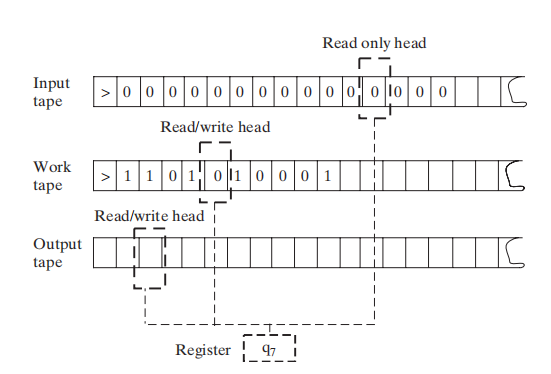
\includegraphics[width=0.8\textwidth]{../images/ComputationalComplexity/1.png}
\end{center}


\begin{definition}[Computing a function and running time]
Let \(f:\{0,1\}^*\to\{0,1\}\) and let \(T:\N\to\N\) be some functions, and let \(M\) be a Turing
machine. We say that \(M\) \textbf{computes} \(f\) if for every \(x\in\{0,1\}^*\), whenever \(M\) is
initialized to the start configuration on input \(x\), then it halts with \(f(x)\) written on
its output tape. We say \(M\) \textbf{computes \(f\) in \(T(n)\)-time} if its computation on every
input \(x\) requires at most \(T(\abs{x})\) steps
\end{definition}

A function \(T:\N\to\N\) is \textbf{time constructible} if \(T(n)\ge n\) and there is a TM \(M\) that
computes the function \(x\mapsto\lcorner{T(\abs{x})}\) in time \(T(n)\). (\(\lcorner{T(\abs{x})}\)
denotes the binary representation of the number \(T(\abs{x})\)). The restriction \(T(n)\ge n\) is
to allow the algorithm time to read its input.

\begin{proposition}[]
For every \(f:\{0,1\}^*\to\{0,1\}\) and a time-constructible b\(T:\N\to\N\), if \(f\) is
computable in time \(T(n)\) by a TM \(M\) using alphabet \(\Gamma\), then it's computable in time
\(4\log\abs{\Gamma}T(n)\) by a TM \(M\) using the alphabet \(\{0,1,\Box,\rhd\}\).
\end{proposition}

\begin{proof}
Let \(M\) be a TM with alphabet \(\Gamma\), \(k\) tapes and state set \(Q\) that computes the
function \(f\) in \(T(n)\) times. We describe an equivalent TM \(\tilde{M}\) computing \(f\)
with alphabet \(\{0,1,\Box,\rhd\}\), \(k\) tapes and a set \(Q'\) of states.

One can encode any member of \(\Gamma\) using \(\log\abs{\Gamma}\) bits. Thus each of \(\tilde{M}\)'s work
tapes will simply encode one of \(M\)'s tapes: For every cell in \(M\)'s tape we will
have \(\log\abs{\Gamma}\) cells in the corresponding tape of \(\tilde{M}\)

To simulate one step of \(M\), the machine \(\tilde{M}\) will 1. use \(\log\abs{\Gamma}\) steps to
read from each tape the \(\log\abs{\Gamma}\) bits encoding of a symbol of \(\Gamma\) 2. use its state register
to store the symbols read 3. use \(M\)'s transition function to compute the symbols \(M\) writes
and \(M\)'s new state given this information 4. store this information in its state register 5.
use \(\log\abs{\Gamma}\) steps to write the encodings of these symbols on its tapes
\end{proof}

\begin{proposition}[]
\label{prop1.6}
Define a single-tape Turing machine to be a TM that has only one read-write tape. For every
\(f:\{0,1\}^*\to\{0,1\}\) and time-constructible \(T:\N\to\N\) if \(f\) is computable in
time \(T(n)\) by a TM \(M\) using \(k\) tapes, then it is computable in time \(5kT(n)^2\) by a
single-tape TM \(M\)
\end{proposition}

\begin{proof}
The TM \(\tilde{M}\) encodes \(k\) tapes of \(M\) on a single tape by using
locations \(1,k+1,2k+1,\dots\) to encode the first tape, locations \(2,k+2,2k+2,\dots\) to
encode the second tape etc. For every symbol \(a\) in \(M\)'s alphabet, \(\tilde{M}\) will
contain both the symbol \(a\) and the symbol \(\hat{a}\). In the encoding of each tape, exactly
one symbol will be of the ``\^{} type'', indicating that the corresponding head of \(M\) is
positioned in that location. \(\tilde{M}\) will not touch the first \(n+1\) locations of its
tape (where the input is located) but rather start by taking \(O(n^2)\) steps to copy the input
bit by bit into the rest of the tape, while encoding it in the above way.
\end{proof}

\begin{remark}[Oblivious Turing machines]
One can ensure that the proof of Proposition \ref{prop1.6} yields a TM \(\tilde{M}\) with the
following property: its head movements do not depend on the input but only depend on the input
length. That is, every input \(x\in\{0,1\}^*\) and \(i\in\N\), the location of each of \(M\)'s
at the \(i\)th step of execution on input \(x\) is only a function of \(\abs{x}\) and \(i\). A
machine with this property is called \textbf{oblivious}.
\end{remark}

\begin{proposition}[]
Define a bidirectional TM to be a TM whose tapes are infinite in both directions. For
every \(f:\{0,1\}^*\to\{0,1\}^*\) and time-constructible \(T:\N\to\N\) if \(f\) is computable in
time \(T(n)\) by a directional TM M, then it is computable in time \(4T(n)\) by a standard
(undirectional) TM \(\tilde{M}\)
\end{proposition}

\begin{proof}
\begin{center}
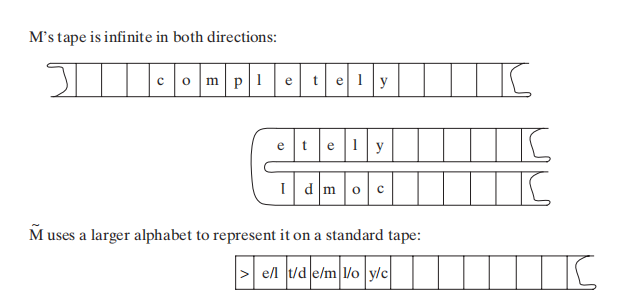
\includegraphics[width=.5\textwidth]{../images/ComputationalComplexity/2.png}
\end{center}

If \(M\) uses alphabet \(\Gamma\), then \(\tilde{M}\) will use the alphabet \(\Gamma^2\) 
\end{proof}

\subsubsection{Machines as Strings and the Universal Turing Machine}
\label{sec:org551d478}
We will also find it convenient to assume that our representation scheme satisfies the following
properties:
\begin{enumerate}
\item We will also find it convenient to assume that our representation scheme satisfies the
following properties:
\item Every TM is represented by infinitely many strings
\end{enumerate}

We denote by \(\lcorner{M}\) the TM \(M\)'s representation as a binary string. If \(\alpha\) is a string
then \(M_\alpha\) denotes the TM that \(\alpha\) represents.

\begin{theorem}[Efficient universal Turing machine]
\label{thm1.9}
There exists a TM \(\calu\) s.t. for
every \(x,\alpha\in\{0,1\}^*\), \(\calu(x,\alpha)=M_\alpha(x)\). Moreover, if \(M_{\alpha}\) halts on
input \(x\) within \(T\) steps then \(\calu(x,\alpha)\) halts within \(CT\log T\) steps, where \(C\)
is a number independent of \(\abs{x}\) and depending only on \(M_\alpha\)'s alphabet size,
number of tapes and number of states.
\end{theorem}

\begin{proof}[Proof of relaxed version of theorem \ref{thm1.9}]
We assume \(M\) has a single work tape (in addition to the input and output tape) and uses he
alphabet \(\{\rhd,\Box,0,1\}\). The reason is that \(\calu\) can transform a representation of
every TM \(M\) into a representation of an equivalent TM \(\tilde{M}\) that satisfies these
properties. (which my takes \(C'T^2\) time)

\begin{figure}[htbp]
\centering
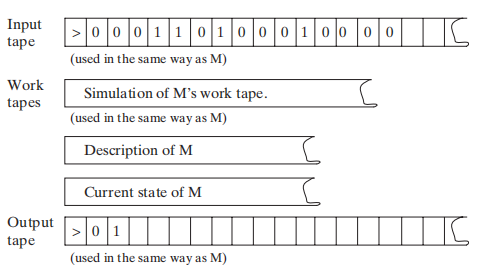
\includegraphics[width=.5\textwidth]{../images/ComputationalComplexity/3.png}
\end{figure}
\end{proof}


\subsubsection{Uncomputablity: An Introduction}
\label{sec:orgfb68dbb}
\begin{theorem}[]
There exists a function \(\text{UC}:\{0,1\}^*\to\{0,1\}\) that is not computable by any TM
\end{theorem}

\begin{proof}
For every \(\alpha\in\{0,1\}^*\), if \(M_{\alpha}(\alpha)=1\) then \(\text{UC}(\alpha)=0\);
otherwise \(\text{UC}(\alpha)=1\).

If its computable, then there exists a TM \(M\) s.t. \(M(\alpha)=\text{UC}(\alpha)\), then
\(M(\lcorner{M})=\text{UC}(\lcorner{M})\)
\end{proof}

\begin{theorem}[]
\(\HALT\) is not computable by any TM
\end{theorem}

\subsubsection{The Class \texorpdfstring{\(P\)}{P}}
\label{sec:orgd2b86b7}
A \textbf{complexity class} is a set of function that can be computed within given resource bounds.

\index{decide}
We say that a machine \textbf{decides} a language \(L\subseteq\{0,1\}^*\) if it computes the
function \(f_L:\{0,1\}^*\to\{0,1\}\) where \(f_L(x)=1\Leftrightarrow x\in L\)

\begin{definition}[]
Let \(T:\N\to\N\) be some function. A language \(L\) is in \(\DTIME(T(n))\) iff there is a
Turing machine that runs in \(c\dot T(n)\) for some constant \(c>0\) and decides \(L\).
\end{definition}

The D in \(\DTIME\) refers to ``deterministic''.

\begin{definition}[]
\(\bP=\bigcup_{c\ge1}\DTIME(n^c)\)
\end{definition}

\subsection{2: NP and NP completeness}
\label{sec:org7718105}

\subsubsection{The Class \(\NP\)}
\label{sec:orged8d120}
\index{$\NP$}
\begin{definition}[]
A language \(L\subseteq\{0,1\}^*\) is in \(\NP\) if there exists  a polynomial \(p:\N\to\N\)
and a polynomial-time TM \(M\) (called the \textbf{verifier} for \(L\)) s.t. for
every \(x\in\{0,1\}^*\)
     \begin{equation*}
x\in L\Leftrightarrow \exists u\in\{0,1\}^{p(\abs{x})}\text{ s.t. }M(x,u)=1
     \end{equation*}
If \(x\in L\) and \(u\in\{0,1\}^{p(\abs{x})}\) satisfy \(M(x,u)=1\) then we call \(u\) a
\textbf{certificate} for \(x\)
\end{definition}

\begin{examplle}[\(\INDSET\in\NP\)]
By representing the possible invitees to a dinner party with the vertices of a graph having an
edge between any two people who don't get along. The dinner party computational problem becomes
the problem of finding a maximum sized \textbf{independent set} (set of vertices without any common
edges) in a given graph. The corresponding language is
     \begin{equation*}
\INDSET=\{\la G,k\ra:\exists S\subseteq V(G)\text{ s.t. }\abs{S}\ge k\text{ and }\forall u,v\in S, \ove{uv}\not\in E(G)\}
     \end{equation*}

Consider the following polynomial-time algorithm \(M\): Given a pair \(\la G,k\ra\) and a
string \(u\in\{0,1\}^*\), output 1 iff \(u\) encodes a list of \(k\) vertices of \(G\) s.t.
there is no edge between any two members of the list. Note that if \(n\) is the number of
vertices in \(G\), then a list of \(k\) vertices can be encoded using \(O(k\log n)\) bits,
where \(n\) is the number of vertices in \(G\). Thus \(u\) is a string of at
most \(O(n\log n)\) bits, which is polynomial in the size of the representation of \(G\).
\end{examplle}

\begin{proposition}[]
Let \(\EXP=\bigcup_{c>1}\DTIME(2^{n^c})\). Then \(\bP\subseteq\NP\subseteq\EXP\)
\end{proposition}

\begin{proof}
\(\bP\subseteq\NP\). Suppose \(L\in\bP\) is decided in polynomial-time by a TM \(N\).
Then we take \(N\) as the machine \(M\) and make \(p(x)\) the zero polynomial

\(\NP\subseteq\EXP\). We can decide \(L\) in time \(2^{O(p(n))}\)  by enumerating all
possible \(n\) and using \(M\) to check whether \(u\) is a valid certificate for the
input \(x\). Note that \(p(n)=O(n^c)\) for some \(c>1\), the number of choices for \(u\) is \(2^{O(n^c)}\).
\end{proof}

\(\NP\) stands for \textbf{nondeterministic polynomial time}.

NDTM has \textbf{two} transition function \(\delta_0\) and \(\delta_1\), and a special state denoted
by \(q_{\accept}\). When an NDTM \(M\) computes a function, we envision that at each
computational step \(M\) makes an arbitrary choice at to which of its two transition functions
to apply. For every input \(x\), we say that \(M(x)=1\) if there \textbf{exists} some sequence of this
choices that would make \(M\) reach \(q_{\accept}\) on input \(x\). We say that \(M\) runs
in \(T(n)\) time if for every input \(x\in\{0,1\}^*\) and every sequence of nondeterministic
choices, \(M\) reaches the halting state or \(q_{\accept}\) within \(T(\abs{x})\) steps

\begin{definition}[]
For every function \(f:\N\to\N\) and \(L\subseteq\{0,1\}^*\) we say that \(L\in\NTIME(T(n))\)
if there is a constant \(c>0\) and a \(c\dot T(n)\)-time NDTM \(M\) s.t. for
every \(x\in\{0,1\}^*\), \(x\in L\Leftrightarrow M(x)=1\)
\end{definition}

\begin{theorem}[]
\(\NP=\bigcup_{c\in\N}\NTIME(n^c)\)
\end{theorem}

\begin{proof}
The main idea is that the sequence of nondeterministic choices made by an accepting computation
of an NDTM can be viewedas a certificate that the input is in the language, and vice versa

Suppose \(p:\N\to\N\) is a polynomial and \(L\) is decidable by a NDTM \(N\) that runs in
time \(p(n)\). For every \(x\in L\), there is a sequence of nondeterministic choices that
makes \(N\) reach \(q_{\accept}\) on input \(x\). We can use this sequence as a certificate
for \(x\). This certificate has length \(p(\abs{x})\) and can be verified in polynomial time by
a deterministic machine.

Conversely, if \(L\in\NP\), then we describe a polynomial time NDTM \(N\) that decides \(L\).
On input \(x\), it uses the ability to make nondeterministic choices to write down a
string \(u\) of length \(p(\abs{x})\). (Having transition \(\delta_0\) correspond to writing a
0 and \(\delta_1\) ). Then it runs the deterministic verifier 
\end{proof}

\subsubsection{Reducibility and NP-Completeness}
\label{sec:org0725b0e}
\begin{definition}[]
A language \(L\subseteq\{0,1\}^*\) is \textbf{polynomial-time Karp reducible to a
language} \(L'\subseteq\{0,1\}^*\) (sometimes shortened to just ``polynomial-time reducible''), denoted
by \(L\le_p L'\) if there is a polynomial-time
computable function \(f:\{0,1\}^*\to\{0,1\}^*\) s.t. for every \(x\in\{0,1\}^*\),
\(x\in L\) iff \(f(x)\in L'\)

We say that \(L'\) is \textbf{\(\NP\)-hard} if \(L\le_pL'\) for every \(L\in\NP\). We say that \(L'\)
is \textbf{\(\NP\)-complete} if \(L'\) is \(\NP\)-hard and \(L'\in\NP\)
\end{definition}

\begin{theorem}[]
\begin{enumerate}
\item (Transitivity) If \(L\le_pL'\) and \(L'\le_pL''\) then \(L\le_pL''\)
\item If language \(L\) is \(\NP\)-hard and \(L\in\bP\) then \(\bP=\NP\)
\item If language \(L\) is \(\NP\)-complete, then \(L\in\bP\) iff \(\bP=\NP\)
\end{enumerate}
\end{theorem}

\begin{theorem}[]
The following language is \(\NP\)-complete
    \begin{equation*}
\TMSAT=\{\la\alpha,x,1^n,1^t\ra:\exists u\in\{0,1\}^n\text{ s.t. }M_\alpha\text{ outputs }1
\text{ on input }\la x,u\ra\text{ within }t\text{ steps}\}
    \end{equation*}
\end{theorem}

\begin{proof}
There is a polynomial \(p\) and a verifier TM \(M\) s.t. \(x\in L\) iff there is a
string \(u\in\{0,1\}^{p(\abs{x})}\) satisfying \(M(x,u)=1\) and \(M\) runs in time \(q(n)\) for
some polynomial \(q\).

Map every string \(x\in\{0,1\}^*\) to the tuple \(\la\lcorner{M},x,1^{p(\abs{x})},1^{q(m)}\)
where \(m=\abs{x}+p(\abs{x})\) and \(\lcorner{M}\) denotes the representation of \(M\) as
string.
    \begin{align*}
&\la\lcorner{M},x,1^{p(\abs{x})},1^{q(m)}\ra\in\TMSAT\\
&\Leftrightarrow\exists u\in\{0,1\}^{p(\abs{x})}\text{ s.t. }M(x,u)\text{ outputs 1 within }q(m)\text{ steps}\\
&\Leftrightarrow x\in L
    \end{align*}
\end{proof}

\subsubsection{The Cook-Levin Theorem: Computation is Local}
\label{sec:orga29e5bf}
We denote by \(\SAT\) the language of all satisfiable CNF formulae and by \(\TSAT\) the
language of all satisfiable 3CNF formulae

\begin{theorem}[Cook-Levin Theorem]
\label{thm2.10}
\begin{enumerate}
\item \(\SAT\) is \(\NP\)-complete
\item \(\TSAT\) is \(\NP\)-complete
\end{enumerate}
\end{theorem}

\begin{lemma}[Universality of AND, OR, NOT]
\label{lemma2.13}
For every Boolean function \(f:\{0,1\}^l\to\{0,1\}\), there is an \(l\)-variable CNF formula \(\varphi\)
of size \(l2^l\) s.t. \(\varphi(u)=f(u)\) for every \(u\in\{0,1\}^l\), where the size of a CNF
formula is defined to be the number of \(\wedge/\vee\) symbols it contains
\end{lemma}

\begin{proof}
For every \(v\in\{0,1\}^l\), there exists a clause \(C_v(z_1,\dots,z_l)\) s.t. \(C_v(v)=0\)
and \(C_v(u)=1\) for every \(u\neq v\).

We let \(\varphi\) be the AND of all the clauses \(C_v\) for \(v\) s.t. \(f(v)=0\)
     \begin{equation*}
\varphi=\bigwedge_{v:f(v)=0}C_v(z_1,\dots,z_l)
     \end{equation*}
Note that \(\varphi\) has size at most \(l2^l\).
\end{proof}

\begin{lemma}[]
\(\SAT\) is \(\NP\)-hard
\end{lemma}

\begin{proof}
Let \(L\) be an \(\NP\) language. By definition, there is a polynomial time TM \(M\) s.t. for
every \(x\in\{0,1\}^*\), \(x\in L\Leftrightarrow M(x,u)=1\) for
some \(u\in\{0,1\}^{p(\abs{x})}\), where \(p:\N\to\N\) is some polynomial. We show \(L\) is
polynomial-time Karp reducible to \(\SAT\) by describing a polynomial-time
transformation \(x\to\varphi_x\) from strings to CNF formulae s.t. \(x\in L\) iff \(\varphi_x\)
is satisfiable. Equivalently
     \begin{equation*}
\varphi_x\in\SAT \quad\text{ iff }\quad\exists u\in\{0,1\}^{p(\abs{x})}
\text{ s.t. }M(x\circ u)=1
     \end{equation*}
where \(\circ\) denotes concatenation

Assume \(M\)
\begin{enumerate}
\item \(M\) only has two tapes - an input tape and a work/output tape
\item \(M\) is an oblivious TM in the sense that its head movement does not depend on the contents
of its tapes. That is, \(M\)'s computation takes the same time for all inputs of size \(n\),
and for every \(i\) the location of \(M\)'s head at the \(i\)th step depends only on \(i\)
and the length of the input
\end{enumerate}


We can make these assumptions without loss of generality because for every \(T(n)\)-time TM \(M\)
there exists a two-tape oblivious TM \(\tilde{M}\) computing the same function
in \(O(T(n)^2)\). Thus in particular, if \(L\in\NP\), then there exists a two-tape oblivious
polynomial-time TM \(M\) and a polynomial \(p\) s.t.
     \begin{equation}
     \label{eq:2.2}
x\in L \Leftrightarrow \exists u\in\{0,1\}^{p(\abs{x})}\text{ s.t. }M(x\circ u)=1
     \end{equation}

Note that because \(M\) is oblivious, we can run it on the trivial input \((x,0^{p(\abs{x})})\)
to determine the precise head position of \(M\) during its computation on every other input of
the same length.

Denote by \(Q\) the set of \(M\)'s possible states and by \(\Gamma\) its alphabet. The \textbf{snapshot}
of \(M\)'s execution on some input \(y\) at a particular step \(i\) is the triple
\(\la a,b,q\ra\in\Gamma\times\Gamma\times Q\) s.t. \(a,b\) are the symbols read by \(M\)'s
heads from the two tapes and \(q\) is the state \(M\) is in at the \(i\)th step. Clearly the
snapshot can be encoded as a binary string. Let \(c\) denote the length of this string, which
is some constant depending upon \(\abs{Q}\) and \(\abs{\Gamma}\)

\begin{figure}[htbp]
\centering
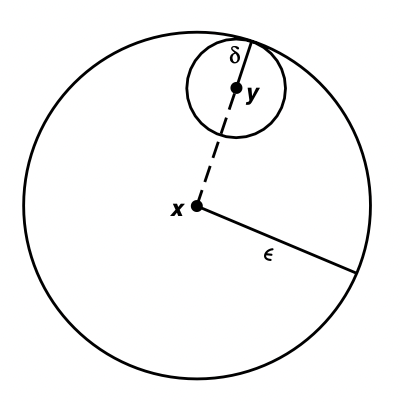
\includegraphics[width=.5\textwidth]{/Users/wu/notes/images/ComputationalComplexity/4.png}
\end{figure}

For every \(y\in\{0,1\}^*\), the snapshot of \(M\)'s execution on input \(y\) at the \(i\)th
step depends on its state in the \((i-1)\)st step and the contents of the current cells of its
input and work tapes.

Suppose somebody were to claim the existence of some \(u\) satisfying \(M(x\circ u)=1\) and as
evidence, present you with the sequence of snapshots that arise from \(M\)'s execution
on \(x\circ u\). How can you tell that the snapshots present a valid computation that was
actually performed by \(M\).

Clearly, it suffices to check that for each \(i\le T(n)\), the snapshot \(z_i\) is correct
given the snapshot for the previous \(i-1\) steps. However, since the TM can only read/modify
one bit at a time, to check the correctness of \(z_i\) it suffices to look at only \emph{two} of the
previous snapshots. Specifically, to check \(z_i\) we need to only look at the following:
\(z_{i-1}\), \(y_{\text{inputpos}(i)}\), \(z_{\text{prev}(i)}\). 

\begin{figure}[htbp]
\centering
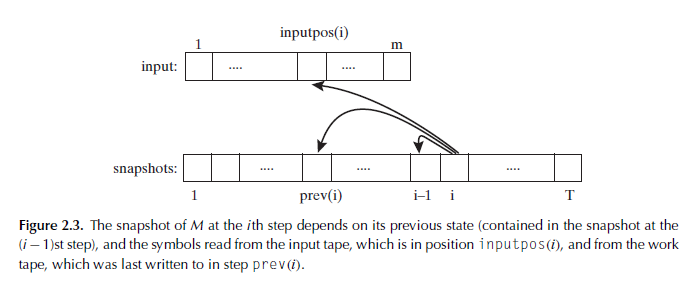
\includegraphics[width=.8\textwidth]{../images/ComputationalComplexity/5.png}
\end{figure}

Here \(y\) is a shorthand
for \(x\circ u\). \(\text{inputpos}(i)\) denotes the location of \(M\)'s input tape head at
the \(i\)th step. \(\text{prev}(i)\) is the last step before \(i\) when \(M\)'s head was in the
same cell on its work tape that it is during step \(i\). The reason this small amount of
information suffices to check the correctness of \(z_i\) is that the contents of the current
cell have not been affected between step \(\text{prev}(i)\) and step \(i\).

Since \(M\) is a deterministic TM, for every triple of values
to \(z_{i-1},y_{\text{inputpos}(i)}\), \(z_{\text{prev}(i)}\), there is at most one value
of \(z_i\) that is correct. Thus there is some function \(F\) that maps \(\{0,1\}^{2c+1}\)
to \(\{0,1\}^c\) s.t. a correct \(z_i\) satisfies
     \begin{equation*}
z_i=F(z_{i-1},z_{\text{prev}(i)},y_{\text{inputpos}(i)})
     \end{equation*}

Because \(M\) is oblivious, the values \(\text{inputpos}(i)\) and \(\text{prev}(i)\) do not
depend on the particular input \(i\). These indices can be computed in polynomial-time by
simulating \(M\) on a trivial input.

By \eqref{eq:2.2} , \(x\in\{0,1\}^{n}\in L\) iff \(M(x\circ u)=1\) for
some \(u\in\{0,1\}^{p(n)}\). The previous discussion shows this latter condition occurs iff
there exists a string \(y\in\{0,1\}^{n+p(n)}\) and a sequence of strings
\(z_1,\dots,z_{T(n)}\in\{0,1\}^c\) (where \(T(n)\) is the number of steps \(M\) takes on inputs
of length \(n+p(n)\)) satisfying the following four conditions
\begin{enumerate}
\item The first \(n\) bits of \(y\) are equal to \(x\)
\item The string \(z_1\) encodes the initial snapshot of \(M\). That is, \(z_1\) encodes the
triple \(\la\rhd,\Box,q_{\start}\ra\).
\item For every \(i\in\{2,\dots,T(n)\}\), \(z_i=F(z_{i-1},z_{\text{prev}(i)},y_{\text{inputpos}(i)})\).
\item The last string \(z_{T(n)}\) encodes a snapshot where the machine halts and outputs 1
\end{enumerate}


The formula \(\varphi_x\) will take variables \(y\in\{0,1\}^{n+p(n)}\)
and \(z\in\{0,1\}^{cT(n)}\) and will verify that \(y,z\) satisfy the AND of these four
conditions. Thus \(x\in L\Leftrightarrow\varphi_x\in\SAT\).

Condition 1 can be expressed as a CNF formula of size \(4n\) . Conditions 2 and 4 each depend
on \(c\) variables and hence by Proposition \ref{lemma2.13} can be expressed by CNF formulae of
size \(c2^c\). Condition 3, which is an AND of \(T(n)\) conditions each  depending on at most \(3c+1\)
variables, can be expressedas a CNF formula of size at most \(T(n)(3c+1)2^{3c+1}\). Hence the AND of all
these conditions can be expressed as a CNF formula of size d(n + T(n)) where d is some constant
depending only on \(M\). Moreover, this CNF formula can be computedin time polynomial in the running
time of \(M\).
\end{proof}

\begin{lemma}[]
\(\SAT\le_p\TSAT\)
\end{lemma}

\begin{proof}
Suppose \(\varphi\) is a 4CNF. Let \(C\) be a clause of \(\varphi\), say \(C=u_1\vee\baru_2\vee\baru_3\vee u_4\).
We add a new variable \(z\) to the \(\varphi\) and replace \(C\) with the pair
\(C_1=u_1\vee\baru_2\vee z\) and \(C_2=\baru_3\vee u_4\vee\barz\). If \(C\) is true, then there
is an assignment to \(z\) that satisfies both \(C_1\) and \(C_2\). If \(C\) is false, then no
matter what value we assign to \(z\) either \(C_1\) or \(C_2\) will be false.

For every clause \(C\) of size \(k>3\), we change it into an equivalent pair of clauses \(C_1\)
of size \(k-1\) and \(C_2\) of size 3.
\end{proof}


\subsubsection{The Web of Reductions}
\label{sec:org98d0336}
\begin{figure}[htbp]
\centering
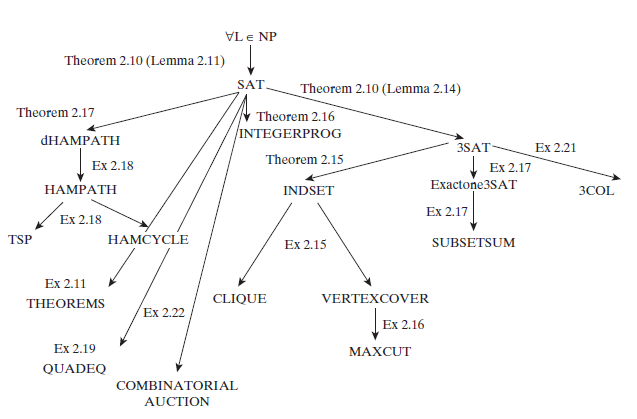
\includegraphics[width=.9\linewidth]{../images/ComputationalComplexity/6.png}
\end{figure}

\begin{theorem}[]
\(\INDSET\) is \(\NP\)-complete
\end{theorem}

\begin{proof}
Transform in polynomial time every \(m\)-clause 3CNF formula \(\varphi\) into a \(7m\)-vertex graph \(G\)

\begin{figure}[htbp]
\centering
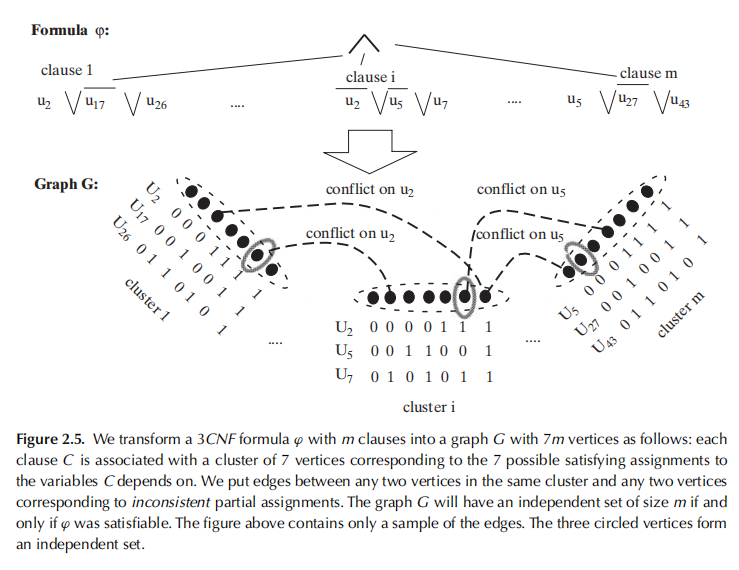
\includegraphics[width=.9\linewidth]{../images/ComputationalComplexity/7.png}
\end{figure}

We associate a cluster of 7 vertices in \(G\) with each clause of \(\varphi\). The vertices in a cluster
associated with a clause \(C\) correspond to the seven possible satisfying partial assignments
to the three variables on which \(C\) depends. For example, if \(C\)
is \(\baru_2\vee\baru_5\vee u_7\), then the seven vertices in the cluster associated with \(C\)
correspond to all partial assignments of the form \(u_1=a,u_2=b,u_3=c\) for a binary
vector \(\la a,b,c\ra\neq\la1,1,0\ra\). We put an edge between two vertices of \(G\) if they
correspond to inconsistent partial assignments. In addition, we put edges between every two
vertices that are in the same cluster

\(\varphi\) is satisfiable iff \(G\) has an independent set of size \(m\)
\end{proof}

We let \(\ZOIPROG\) be the set of satisfiable 0/1 integer programs.
That is, a set of linear inequalities with rational coefficients over
variables \(u_1,\dots,u_n\) is in \(\ZOIPROG\) if there is an assignment of numbers in \(\{0,1\}\)
to \(u_1,\dots,u_n\) that satisfies it

\begin{theorem}[]
\(\ZOIPROG\)is \(\NP\)-complete

Every CNF formula can be expressed as an integer program by expressing every clause as
inequality. For example, the clause \(u_1\vee\baru_2\vee\baru_3\) can be expressed by
\(u_1+(1-u_2)+(1-u_3)\ge1\).
\end{theorem}

A \textbf{Hamilton path} in a directed graph is a path that visits all vertices exactly once. Let
\(\dHAMPATH\) denote the set of all directed graphs that contain such a path
\begin{theorem}[]
\(\dHAMPATH\) is \(\NP\)-complete
\end{theorem}

\begin{proof}
\begin{figure}[htbp]
\centering
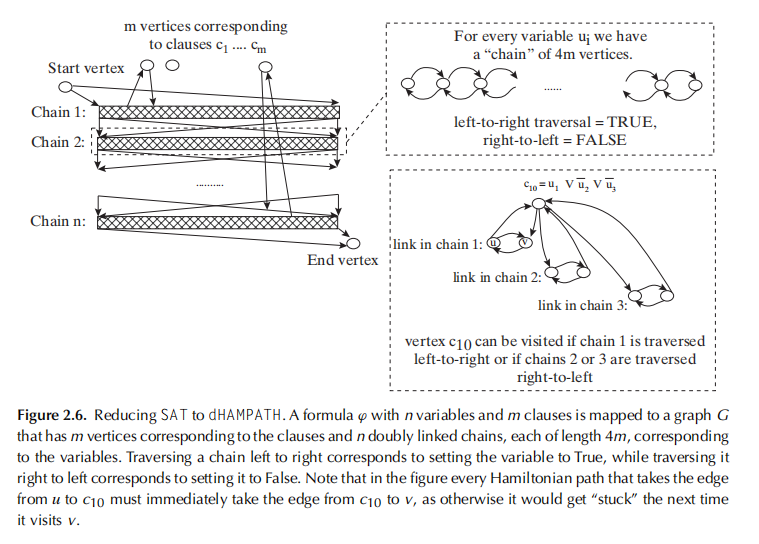
\includegraphics[width=.9\linewidth]{../images/ComputationalComplexity/8.png}
\end{figure}

The graph \(G\) has
\begin{enumerate}
\item \(m\) vertices for each of \(\varphi\)'s clause \(c_1,\dots,c_m\)
\item a special starting vertex \(v_{\start}\) and ending vertex \(v_{\tend}\)
\item \(n\) ``chains'' of \(4m\) vertices corresponding to the \(n\) variables of \(\varphi\) . A chain is a
set of vertices \(v_1,\dots,v_{4m}\) s.t. for every \(i\in[1,4m-1]\), \(v_i\)
and \(v_{i+1}\) are connected by two edges in both directions
\end{enumerate}


If \(C\) contains the literal \(u_j\), then we take two neighboring
vertices \(v_i\), \(v_{i+1}\) in the \(j\)th chain and put an edge from \(v_i\) to \(C\) and
from \(C\) to \(v_{i+1}\). If \(C\) contains the literal \(\baru_j\) then we construct these
edges in the opposite direction. When adding these edges, we never ``reuse'' a
link \(v_i, v_{i+1}\) in a particular chain and always keep an unused link between every two
used links.


\(G\in\dHAMPATH\Rightarrow\varphi\in\SAT\). Suppose that \(G\) has an Hamiltonian path \(P\).
We first note that the path \(P\) must start in \(v_{\start}\) and end at \(v_{\tend}\).
Furthermore, we claim that \(P\) needs to traverse all the chains in order and, within each
each chain, traverse it either in left-to-right order or right-to-left order.
\end{proof}

\subsubsection{Decision versus Search}
\label{sec:org6623626}
\begin{theorem}[]
\label{thm2.18}
Suppose that \(\bP=\NP\). Then for every \(\NP\) language \(L\) and a verifier TM \(M\)
for \(L\), there is a polynomial-time TM \(B\) that on input \(x\in L\) outputs a certificate
for \(x\).
\end{theorem}

\begin{proof}
We need to show that if \(\bP=\NP\) then for every polynomial-time TM \(M\) and
polynomial \(p(n)\), there is a polynomial-time TM \(B\) with the following property: for every
\(x\in\{0,1\}^n\) if there is \(u\in\{0,1\}^{p(n)}\) s.t. \(M(x,u)=1\) then \(\abs{B(x)}=p(n)\)
and \(M(x,B(x))=1\)

We start by showing the theorem for the case of \(\SAT\). In particular, we show that given an
algorithm \(A\) that decides \(\SAT\), we can come up an algorithm \(B\) that on input a
satisfiable CNF formula \(\varphi\) with \(n\) variables, finds a satisfying assignment for \(\varphi\)
using \(2n+1\) calls to \(A\) and some additional polynomial-time computation.

We first use \(A\) to check that the input formula is satisfiable. If so, we first
substitute \(x_1=0\) and then \(x_1=1\) in \(\varphi\) and then use \(A\) to decide which of the two is
satisfiable. Say the first is satisfiable. Then we fix \(x_1=0\). Continuing this way, we end
up with an assignment

To solve the search problem for an arbitrary \(\NP\)-language \(L\), we use the fact that the
reduction of Theorem \ref{thm2.10} from \(L\) to \(\SAT\)is actually a Levin reduction. This
means that we have a polynomial-time computable function \(f\) s.t. we can map a satisfying
assignment of \(f(x)\) into a certificate for \(x\).
\end{proof}

The theorem \ref{thm2.18} shows that \(\SAT\) is \textbf{downward self-reducible}, which means that
given an algorithm that solves \(\SAT\) on inputs of length smaller than \(n\) we can
solve \(\SAT\) on inputs of length \(n\).

\subsubsection{\textbf{CONP,EXP} and \textbf{NEXP}}
\label{sec:org9889929}

\begin{definition}[]
\label{def2.19}
\(\coNP=\{L:\barL\in\NP\}\)
\end{definition}

\begin{definition}[alternative definition]
\label{def2.20}
For every \(L\subseteq\{0,1\}^*\), we say that \(L\in\coNP\) if there exists a
polynomial \(p:\N\to\N\) and a polynomial-time TM \(M\) s.t. for every \(x\in\{0,1\}^*\)
     \begin{equation*}
x\in L \Leftrightarrow\forall u\in\{0,1\}^{p(\abs{x})},\; M(x,u)=1
     \end{equation*}
\end{definition}

\begin{examplle}[]
The following language is \(\coNP\)-complete
     \begin{align*}
\TAUTOLOGY=\{\varphi:\varphi\text{ is a tautology}\}
     \end{align*}
It's clearly in \(\coNP\) by Definition \ref{def2.20} (Make \(u\) to be the all possible
assignments). Modify the Cook-Levin reduction 
from \(\barL\)(which is in \(\NP\)) to \(\SAT\). For every input \(x\in\{0,1\}^*\) that
reduction produces a formula \(\varphi_x\) that is satisfiable iff \(x\in\barL\). Now consider
the formula \(\neg\varphi_x\). It is in \(\TAUTOLOGY\) iff \(x\in L\)
\end{examplle}

\subsubsection{\(\EXP\) and \(\NEXP\)}
\label{sec:orgc3dead4}
\begin{theorem}[]
If \(\EXP\neq\NEXP\) then \(\bP\neq\NP\)
\end{theorem}

\begin{proof}
We prove the contrapositive: Assuming \(\bP=\NP\) we show \(\EXP=\NEXP\).
Suppose \(L\in\NTIME(2^{n^c})\) and NDTM \(M\) decides it. We claim that the language
     \begin{equation*}
L_{\pad}=\left\{\la x,1^{2^{\abs{x}^c}}\ra:x\in L
\right\}
     \end{equation*}
is in \(\NP\). Here is an NDTM for \(L_{\pad}\): Given \(y\), first check if there is a
string \(z\) s.t. \(y=\la z,1^{2^{\abs{z}^c}}\ra\). If not, output 0. If \(y\) is of this form,
then simulate \(M\) on \(z\) for \(2^{\abs{z}^c}\) steps and output its answer. The running
time is polynomial in \(\abs{y}\), and hence \(L_{\pad}\in\NP\). Hence if \(\bP=\NP\)
then \(L_{\pad}\in\bP\). But if \(L_{\pad}\) is in \(\bP\) then \(L\) is in \(\EXP\). To
determine whether an input \(x\) is in \(L\), we just pad the input and decide whether it is
in \(L_{\pad}\) using the polynomial-time machine for \(L_{\pad}\)
\end{proof}


\subsubsection{Exercise}
\label{sec:org661c99d}
\begin{exercise}
\label{ex2.11}
Argue at a high level that the following language is \(\NP\)-complete
     \begin{equation*}
\left\{\la\varphi,1^n\ra:\text{ math statement }\varphi
\text{ has a proof of size at most $n$ in the ZF system}
\right\}
     \end{equation*}
\end{exercise}

\begin{proof}
Essential part is to find a reduction.

Idea: if there are \(n\) derivation rules, then we consider \(n\SAT\)
\end{proof}

\begin{exercise}
\label{ex2.23}
Prove that \(\bP\subseteq\NP\cap\coNP\)
\end{exercise}

\begin{exercise}
\label{ex2.24}
Prove that Definition \ref{def2.19} and \ref{def2.20} do indeed define the same class
\end{exercise}

\begin{proof}
Suppose \(\coNP=\{L:\barL\in\NP\}\).
     \begin{align*}
x\in L\in\coNP& \Leftrightarrow x\not\in\barL\in\NP\\
& \Leftrightarrow\neg\exists u\in\{0,1\}^{p(\abs{x})} M'(x,u)=1\\
&\Leftrightarrow\forall u\in\{0,1\}^{p(\abs{x})}M'(x,u)\neq1\\
&\Leftrightarrow\forall u\in\{0,1\}^{p(\abs{x})}M(x,u)=1\\
     \end{align*}
where \(M'\) is a TM for \(\NP\) and \(M\) is a TM for \(\coNP\) by computing the value
from \(M'\).

Another direction is the same.
\end{proof}

\subsection{4: Space Complexity}
\label{sec:org8723600}
\subsubsection{Definition of Space-Bounded Computation}
\label{sec:org3d41438}
TM we use is
\begin{figure}[htbp]
\centering
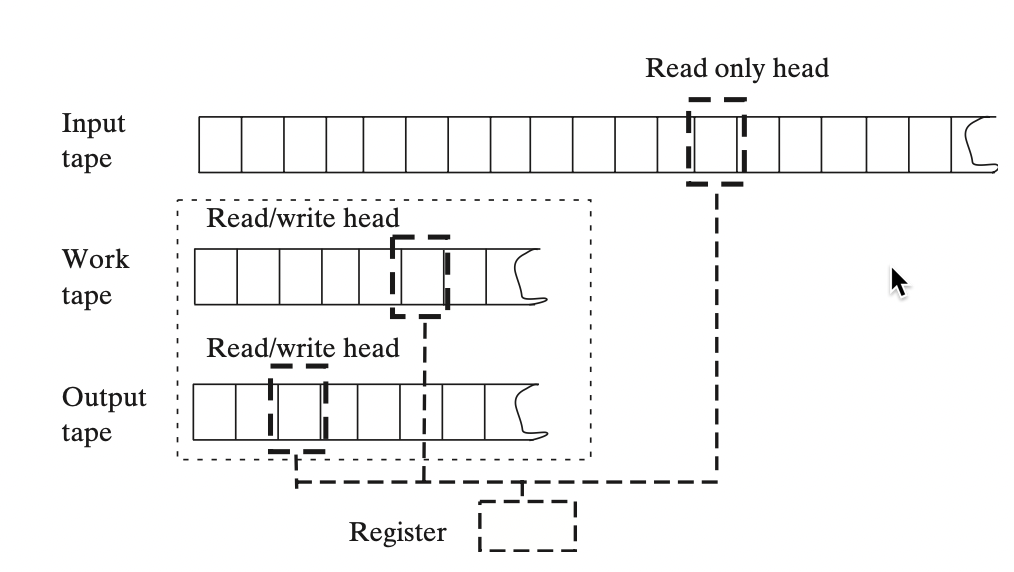
\includegraphics[width=.7\textwidth]{../images/ComputationalComplexity/9.png}
\label{}
\end{figure}

\begin{definition}[Space-bounded computation]
Let \(S:\N\to\N\) and \(L\subseteq\{0,1\}^*\). We say that \(L\in\SPACE(s(n))\) if there is a
constant \(c\) and a TM \(M\) deciding \(L\) s.t. at most \(c\cdot s(n)\) locations on \(M\)'s
work tapes (excluding the input tape) are ever visited by \(M\)'s head during its computation on
every input of length \(n\)

Similarly we say that \(L\in\NSPACE(s(n))\) if there is an NDTM \(M\) deciding \(L\) that never
uses more than \(c\cdot s(n)\) nonblank tape locations on length \(n\) inputs
\end{definition}



\(S:\N\to\N\) is \textbf{space-constructible} if there is a TM that computes \(S(\abs{x})\)
in \(O(S(\abs{x}))\) space given \(x\) as input

Since the TM's work tapes are separated from its input tape, it makes sense to consider
space-bounded machines that use space less than the input length, namely, \(S(n)<n\). We will
require however that \(S(n)>\log n\).

\(\DTIME(S(n))\subseteq\SPACE(S(n))\) since a TM can access only one tape cell per step. But
a \(\SPACE(S(n))\) machine can run for much longer than \(S(n)\) steps

\begin{theorem}[]
\label{thm4.2}
For every space constructible \(S:\N\to\N\)
\begin{equation*}
\DTIME(S(n))\subseteq\SPACE(S(n))\subseteq\NSPACE(S(n))\subseteq\DTIME(2^{O(S(n))})
\end{equation*}
\end{theorem}


We use the notion of a \textbf{configuration graph} of a Turing machine. Let \(M\) be a (deterministic or
nondeterministic) TM. A \textbf{configuration} of a TM \(M\) consists of the contents of all nonblank
entries of \(M\)'s tapes, along with its state and head position, at a particular point in its
execution. For every space \(S(n)\) TM \(M\) and input \(x\in\{0,1\}^*\), the
\textbf{configuration graph of \(M\) on input \(x\)}, denoted \(G_{M,x}\), is a directed graph whose nods
correspond to all possible configuration of \(M\) where the input contains the value \(x\) and
the work tapes have at most \(S(\abs{x})\) nonblank cells. The graph has a directed edge from a
configuration \(C\) to a configuration \(C'\) if \(C'\) can be reached from \(C\) in one step
according to \(M\)'s transition function. By modifying \(M\) to erase all its work tapes before
halting, we can assume that there is only a single configuration \(C_{\accept}\) on which \(M\)
halts and outputs 1.

\begin{claim}
\label{claim4.4}
Let \(G_{M,x}\) be the configuration graph of a space-\(S(n)\) machine \(M\) on some
 input \(x\) of length \(n\). Then
\begin{enumerate}
\item Every vertex in \(G_{M,x}\) can be described using \(cS(n)\) bits for some constant \(c\)
(depending on \(M\)'s alphabet size and number of tapes') and in particular, \(G_{M,x}\) has
at most \(2^{cS(n)}\) nodes
\item There is an \(O(S(n))\)-size CNF formula \(\varphi_{M,x}\) s.t. for every two
strings \(C,C'\) \(\varphi_{M,x}(C,C')=1\) iff \(C\) and \(C'\) encodes two neighboring
configuration in \(G_{M,x}\)
\end{enumerate}
\end{claim}

\begin{proof}[proof of theorem \ref{thm4.2}]
By enumerating all possible configurations, we can construct the graph \(G_{M,x}\)
in \(2^{O(S(n))}\)-times  and check whether \(C_{\start}\) is connected to \(C_{\accept}\)
in \(G_{M,x}\) using the standard breadth-first search algorithm for connectivity
\end{proof}

\begin{definition}[]
\begin{align*}
\PSPACE&=\bigcup_{c>0}\SPACE(n^c)\\
\NPSPACE&=\bigcup_{c>0}\NSPACE{n^c}\\
\bL&=\SPACE(\log n)\\
\NL&=\NSPACE(\log n)
\end{align*}
\end{definition}

\begin{examplle}[]
\(\TSAT\in\PSPACE\). The machine just uses the linear space to cycle through all \(2^k\)
assignments to order. Once an assignment is checked, erase it on tape.

In fact, \(\NP\subseteq\PSPACE\).
\end{examplle}

Let
\begin{center}
\(\PATH=\{\la G,s,t\ra:G\) is a directed graph in which there is a path from \(s\) to \(t\}\)
\end{center}
Note that  \(\PATH\in\NL\).

\begin{theorem}[Space Hierarchy Theorem]
If \(f,g\) are space-constructible functions satisfying \(f(n)=o(g(n))\), then
\begin{equation*}
\SPACE(f(n))\subsetneq\SPACE(g(n))
\end{equation*}
\end{theorem}
\subsubsection{\(\PSPACE\) Completeness}
\label{sec:org057fb51}
\begin{definition}[]
A language \(L'\) is \textbf{\(\PSPACE\)-hard} if for every \(L\in\PSPACE\), \(L\le_p L'\). If in
addition \(L'\in\PSPACE\) then \(L'\) is \textbf{\(\PSPACE\)-complete}
\end{definition}

\begin{definition}[Quantified Boolean Formula]
A \textbf{quantified Boolean formula} (QBF) is a formula of the form \(Q_1x_1\dots Q_nx_n\varphi(x_1,\dots,x_n)\) where
each \(Q_i\)is one of the two quantifiers \(\forall\) or \(\exists\), \(x_1,\dots,x_n\) ranges over \(\{0,1\}\) and
\(\varphi\) is a quantifier-free Boolean formula.
\end{definition}

Let \(\TQBF\) be the set of quantified Boolean formulae that are true
\begin{theorem}[]
\label{thm4.13}
\(\TQBF\) is \(\PSPACE\)-complete
\end{theorem}

\begin{proof}
First we show that \(\TQBF\in\PSPACE\). Let
\begin{equation*}
\psi=Q_1x_1\dots Q_nx_n\varphi(x_1,\dots,x_n)
\end{equation*}
be a quantified Boolean formula with \(n\) variables, where we denote the size of \(\varphi\) by \(m\). We
show a recursive algorithm \(A\) that can decide the truth of \(\psi\) in \(O(n+m)\) space.

If \(n=0\) then \(\varphi\) can be evaluated in \(O(m)\) time and space, and so we assume \(n>0\).
For \(b\in\{0,1\}\) denote by \(\psi\restriction_{x_1=b}\) the modification of \(\psi\) where the first
quantifier \(Q_1\) is dropped and all occurrences of \(x_1\) are replaces with the constant \(b\).
Algorithm \(A\) will works as follows: if \(Q_1=\exists\) then output 1 iff at least one
of \(A(\psi\restriction_{x_1=0})\)  and \(A(\psi\restriction_{x_1=1})\) outputs 1. If \(Q_1=\forall\), then
output 1 iff both  \(A(\psi\restriction_{x_1=0})\)  and \(A(\psi\restriction_{x_1=1})\) outputs 1.

Let \(s_{n,m}\) denote the space \(A\) uses on formula with \(n\) variables and description
size \(m\). The crucial point is - here we use the fact that space can be \textbf{reused} - that both
recursive computations  \(A(\psi\restriction_{x_1=0})\)  and \(A(\psi\restriction_{x_1=1})\) can run in
the same space. Thus assuming that \(A\) uses \(O(m)\) space to
write  \(A(\psi\restriction_{x_1=b})\) for its recursive calls, we'll get that
\(s_{n,m}=s_{n-1,m}+O(m)\) yielding \(s_{n,m}=O(n\cdot m)\)

We now show that \(L\le_p\TQBF\) for every \(L\in\PSPACE\). Let \(M\) be a machine that
decides \(L\) in \(S(n)\) space and let \(x\in\{0,1\}^n\). We show how to construct a quantified
Boolean formula of size \(O(S(n)^2)\) that is true iff \(M\) accepts \(x\). Let \(m=O(S(n))\)
denote the number of bits needed to encode a configuration of \(M\) on length \(n\). By Claim
\ref{claim4.4} there is a Boolean formula \(\varphi_{M,x}\) s.t. for every two
strings \(C,C'\in\{0,1\}^m\) \(\varphi_{M,x}(C,C)=1\) iff \(C\) and \(C'\) encode two adjacent
configurations in the configuration graph \(G_{M,x}\).

let \(\psi_i(C,C')\) be true iff there is a path of length at most \(2^i\) from \(C\) to \(C'\)
in \(G_{M,x}\). Note that \(\psi=\psi_m\) and \(\psi_0=\varphi_{M,x}\). The crucial point is
\(\psi_i(C,C')=\exists C''\psi_{i-1}(C,C'')\wedge\psi_{i-1}(C'',C')\)

But \(\psi_m\) has size about \(2^m\), which is not good. Instead, we use additional quantified
variables to save on description size
\begin{equation*}
\exists C''\forall D_1\forall D_2((D_1=C\wedge D_2=C'')\vee(D_1=C''\wedge D_2=C'))\to \psi_{i-1}(D_1,D_2)
\end{equation*}
Note that \(size(\psi_i)\le size(\psi_{i-1})+O(m)\) and hence \(size(\psi_m)\le o(m^2)\)
\end{proof}

Since we don't require the graph in proof of Theorem \ref{thm4.13} to have out-degree one, it
actually yields a stronger statement
\begin{equation*}
\TQBF\in\NPSPACE
\end{equation*}

\begin{theorem}[Savitch's Theorem]
For any space-constructible \(S:\N\to\N\) with \(S(n)\ge\log n\), \(\NSPACE(S(n))\subseteq\SPACE(S(n)^2)\)
\end{theorem}

\begin{proof}
Let \(L\in\NSPACE(S(n))\) be a language decided by a TM \(M\) s.t. for every \(x\in\{0,1\}^n\), the
configuration graph \(G=G_{M,x}\) has at most \(M=2^{O(S(n))}\) vertices, and determining
whether \(x\in L\)is equivalent to determining whether \(C_{\accept}\) can be reached
from \(C_{\start}\) in this graph. We describe a recursive procedure \(\text{REACH?}(u,v,i)\)
that returns ``YES'' if there is a path from \(u\) to \(v\) of length at most \(2^i\) and ``NO''
otherwise.
\begin{equation*}
\text{REACH?}(u,v,i)=\exists w(\text{REACH?}(u,w,i-1)\vee\text{REACH?}(w,v,i-1))
\end{equation*}
Let \(s_{M,i}\) be the space complexity of \(\text{REACH?}(u,v,i)\),
then \(s_{M,i}=s_{M,i-1}+O(\log M)\) (since we need to enumerate all \(w\) in TM, the space we
need is \(O(\log M)\)) and thus
\(s_{M,\log M}=O(\log^2 M)=O(S(n)^2)\)
\end{proof}

\begin{examplle}[The QBF game]
The ``board'' for the QBF game is a Boolean formula \(\varphi\) whose free variables are \(x_1,\dots,x_{2n}\).
player 1 will pick values for the odd-numbered variables. We say player 1 wins iff at the end
\(\varphi(x_1,\dots,x_{2n})\) is true

In order for player 1 to have a \textbf{winning strategy} he must have a way to win for all possible
sequences of moves by player 2, namely, if
\begin{equation*}
\exists x_1\forall x_2 \exists x_3\forall x_4\dots\forall x_{2n}\varphi(x_1,\dots,x_{2n})
\end{equation*}
Thus deciding whether player 1 has a winning strategy for a given board in the QBF game is \(\PSPACE\)-complete.
\end{examplle}
\subsubsection{\(\NL\) Completeness}
\label{sec:org94d04fc}

We cannot use the polynomial-time reduction since \(\bL\subseteq\NL\subseteq\bP\) (cf. Exercise \ref{ex4.3})

\begin{definition}[logspace reduction and \(\NL\)-completeness]
A function \(f:\{0,1\}^*\to\{0,1\}^*\) is \textbf{implicitly logspace computable}, if \(f\) is polynomially
bounded (i.e., there is some \(c\) s.t. \(\abs{f(x)}\le\abs{x}^c\) for every \(x\in\{0,1\}^*\)) and the
language \(L_f=\{\la x,i\ra\mid f(x)_i=1\}\) and \(L_f'=\{\la x,i\ra\mid i\le\abs{f(x)}\}\) are in \(\bL\)

A language \(B\) is \textbf{logspace reducible} to language \(C\), denoted by \(B\le_lC\) if there is a
function \(f:\{0,1\}^*\to\{0,1\}^*\) that is implicitly logspace computable and \(x\in B\)
iff \(f(x)\in C\) for every \(x\in\{0,1\}^*\).

We say that \(C\) is \textbf{\(\NL\)-complete} if it is in \(\NL\) and for every \(B\in\NL\), \(B\le_lC\)
\end{definition}

Another way(used by several texts) to think of logspace reductions is to imagine that the
reduction is given
a separate ``write-once'' output tape, on which it can either
write a bit or move to the right but never move left or read the bits it wrote down
previously.The two notions are easily proved to be equivalent (seeExercise \ref{ex4.8}).

\begin{lemma}[]
\begin{enumerate}
\item If \(B\le_lC\) and \(C\le_lD\) then \(B\le_lD\)
\item if \(B\le_lC\) and \(C\in\bL\) then \(B\in\bL\)
\end{enumerate}
\end{lemma}

\begin{proof}
We prove that if \(f,g\) are two implicitly logspace computable functions, then so
if \(h(x)=g(f(x))\). Part 2 follows by letting \(f\) be the reduction from \(B\) to \(C\)
and \(g\) be the characteristic function of \(C\) (i.e., \(g(y)=1\) iff \(y\in C\))

Let \(M_f,M_g\) be the logspace machines that compute the mappings \(x,i\mapsto f(x)_i\)
and \(y,j\mapsto g(y)_i\) respectively. We construct a machine \(M_h\) that given input \(x,j\)
with \(j\le\abs{g(f(x))}\) outputs \(g(f(x))_j\)

\begin{figure}[htbp]
\centering
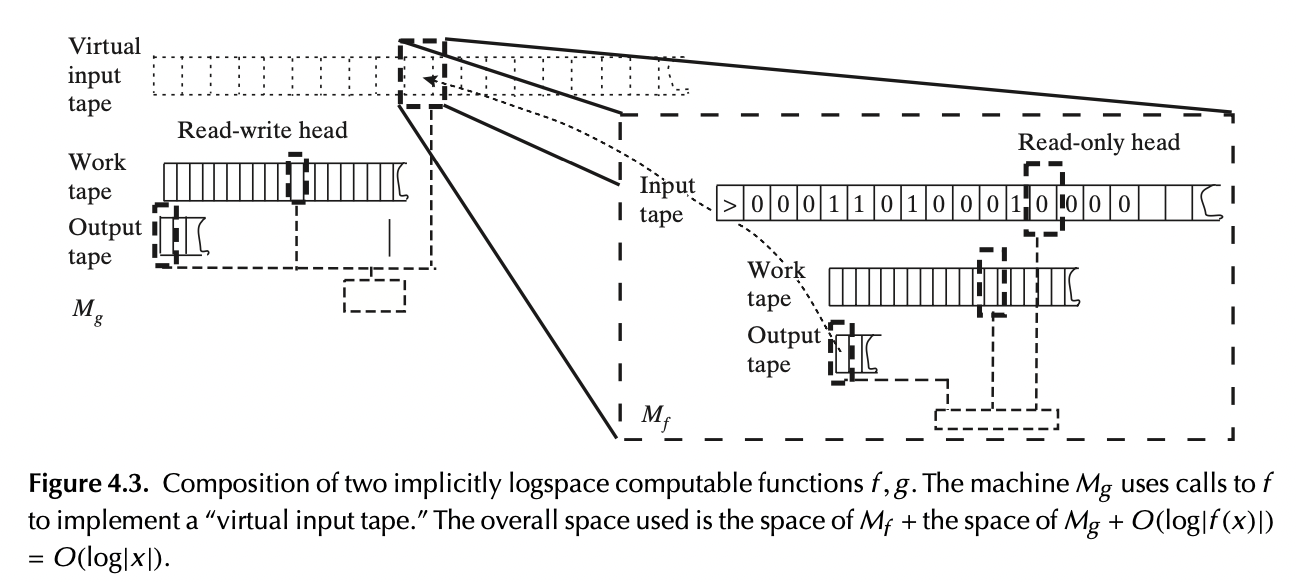
\includegraphics[width=.9\textwidth]{../images/ComputationalComplexity/10.png}
\label{}
\end{figure}
\end{proof}

\subsubsection{Exericse}
\label{sec:org66149ef}
\begin{exercise}
\label{ex4.3}
Prove that every language \(L\) that is not the empty or \(\{0,1\}^*\) is complete for \(\NL\)
under polynomial-time Karp reductions
\end{exercise}

\begin{exercise}
\label{ex4.8}
\end{exercise}
\end{document}
